% =============================================================================
%  Informe de Proyecto — Simulación de Eventos Discretos
%  Problema: Poblado en Evolución
% =============================================================================
\documentclass[12pt, a4paper]{article}

% --- Codificación y lengua ---------------------------------------------------
\usepackage[utf8]{inputenc}
\usepackage[T1]{fontenc}
\usepackage[spanish, es-tabla]{babel}

% --- Geometría y tipografía --------------------------------------------------
\usepackage[top=2.5cm, bottom=2.5cm, left=3cm, right=2.5cm]{geometry}
\usepackage{microtype}
\usepackage{setspace}
\onehalfspacing

% --- Matemáticas -------------------------------------------------------------
\usepackage{amsmath, amssymb}

% --- Tablas ------------------------------------------------------------------
\usepackage{booktabs}
\usepackage{multirow}
\usepackage{array}
\usepackage{float}

% --- Gráficos e hipervínculos ------------------------------------------------
\usepackage{graphicx}
\usepackage[colorlinks=true, linkcolor=black, urlcolor=blue, citecolor=black]{hyperref}

% --- Código fuente -----------------------------------------------------------
\usepackage{listings}
\usepackage{xcolor}

\lstdefinestyle{python}{
  language=Python,
  basicstyle=\ttfamily\small,
  keywordstyle=\color{blue}\bfseries,
  commentstyle=\color{gray}\itshape,
  stringstyle=\color{teal},
  numbers=left,
  numberstyle=\tiny\color{gray},
  stepnumber=1,
  numbersep=6pt,
  backgroundcolor=\color{gray!5},
  frame=single,
  framerule=0.4pt,
  rulecolor=\color{gray!40},
  breaklines=true,
  captionpos=b,
}

% --- Cabeceras ---------------------------------------------------------------
\usepackage{fancyhdr}
\pagestyle{fancy}
\fancyhf{}
\lhead{\small Simulación de Eventos Discretos}
\rhead{\small Poblado en Evolución}
\cfoot{\thepage}
\renewcommand{\headrulewidth}{0.4pt}

% --- Comandos de utilidad ----------------------------------------------------
\newcommand{\Exp}[1]{\mathrm{Exp}\!\left(#1\right)}
\newcommand{\Unif}[2]{\mathrm{Unif}\!\left(#1,\,#2\right)}
\newcommand{\Bern}[1]{\mathrm{Bern}\!\left(#1\right)}
\newcommand{\code}[1]{\texttt{#1}}

% =============================================================================
\begin{document}

% --- Portada -----------------------------------------------------------------
\begin{titlepage}
  \centering
  \vspace*{1.5cm}

  {\Large \textbf{Universidad de La Habana}\\[0.3em]
   \large Facultad de Matemática y Computación}

  \vspace{2cm}
  \rule{\linewidth}{0.5pt}\\[0.4cm]
  {\LARGE \textbf{Simulación de Eventos Discretos}}\\[0.3cm]
  {\large \textit{Poblado en Evolución}}\\[0.2cm]
  \rule{\linewidth}{0.5pt}

  \vspace{1.5cm}

  \begin{tabular}{ll}
    \textbf{Estudiante:}  & {David S\'anchez Iglesias} \\[0.4em]
    \textbf{Grupo:}       & {C411} \\[0.4em]
    \textbf{Asignatura:}  & Simulación \\[0.4em]
    \textbf{Año académico:} & 4.º año, Curso 2025--2026 \\
  \end{tabular}

  \vspace{2cm}

  \textbf{Repositorio GitHub:}\\[0.3em]
  \url{https://github.com/Davidbestion/sim_project}

  \vfill
  {\small La Habana, mayo de 2026}
\end{titlepage}

% --- Índice ------------------------------------------------------------------
\tableofcontents
\newpage

% =============================================================================
\section{Orden del Problema Asignado}
% =============================================================================

El problema abordado se denomina \textit{Poblado en Evolución}.
Su objetivo consiste en determinar cómo evoluciona la población de una región
hipotética a lo largo de un período de cien años, partiendo de una población
inicial de $H$ hombres y $M$ mujeres cuyas edades se distribuyen de forma
uniforme en el intervalo $[0, 100)$ años.

El enunciado provee tablas de probabilidad para modelar:
\begin{enumerate}
  \item La probabilidad de fallecimiento en función de la edad y el sexo.
  \item La probabilidad de embarazo de una mujer según su edad.
  \item El número de hijos deseados por cada individuo.
  \item La probabilidad de querer tener pareja según la edad.
  \item La probabilidad de establecer pareja en función de la diferencia de
        edades entre dos personas.
  \item La dinámica de ruptura y el período de soledad post-ruptura.
  \item La probabilidad de embarazo múltiple y el sexo de los recién nacidos.
\end{enumerate}

% =============================================================================
\section{Principales Ideas Seguidas para la Solución}
% =============================================================================

\subsection{Paradigma de Simulación Seleccionado}

Se adoptó el paradigma de \textit{Simulación de Eventos Discretos}
(SED\footnote{Del inglés \textit{Discrete-Event Simulation} (DES). Ambos
acrónimos se emplean indistintamente en la literatura; en este informe se
utiliza la sigla \textbf{DES} cuando se hace referencia al motor o a las
estructuras de implementación, y \textbf{SED} en el contexto conceptual.}),
en el que el estado del sistema únicamente cambia en instantes puntuales
denominados \textit{eventos}. Entre dos eventos consecutivos, el estado
permanece constante, lo que permite avanzar el reloj de simulación
directamente al siguiente evento sin iterar paso a paso. Este enfoque es
particularmente adecuado para sistemas demográficos, donde la mayoría de
los fenómenos (nacimientos, muertes, formación de parejas) son sucesos
discretos y esporádicos en el tiempo continuo.

\subsection{Implementación}

La implementación se realizó en \textbf{Python 3}, sin dependencias externas
para la generación de variables aleatorias. Todas las distribuciones se
construyen a partir de \code{random.random()}, que genera valores
$U \sim \Unif{0}{1}$, aplicando la transformada inversa o métodos de
aceptación--rechazo cuando corresponde. La cola de prioridad del motor DES
se implementa mediante \code{heapq}, que garantiza complejidad
$\mathcal{O}(\log n)$ por operación de inserción y extracción.

El proyecto se organiza en los siguientes módulos:

\begin{description}
  \item[\code{distributions.py}] Generación de todas las variables
        aleatorias del modelo. Centraliza las tablas de probabilidad del
        enunciado y las funciones de muestreo correspondientes.
  \item[\code{person.py}] Clase \code{Person}, que encapsula el estado
        completo de un individuo: edad, sexo, estado sentimental, número de
        hijos tenidos y deseados, y bandera de embarazo.
  \item[\code{events.py}] Tipos de eventos (\code{EventType}), estructura
        de datos \code{Event} y los \textit{handlers} que implementan la
        lógica de cada tipo de evento.
  \item[\code{simulation.py}] Motor principal: inicializa la población,
        puebla la cola de eventos y ejecuta el bucle DES.
  \item[\code{stats.py}] Recolección de métricas durante la ejecución y
        generación de visualizaciones al finalizar.
  \item[\code{main.py}] Punto de entrada con interfaz de línea de comandos.
  \item[\code{batch\_run.py}] Herramienta de réplicas múltiples para análisis
        estadístico de la variabilidad del modelo.
  \item[\code{gen\_figures.py}] Script auxiliar que ejecuta todos los escenarios
        del análisis (corrida única y 30 réplicas de batch) y genera
        automáticamente las 14 figuras del Anexo~A.
\end{description}

\subsection{Decisiones de Modelado Relevantes}

\paragraph{Tiempo hasta el fallecimiento.}
La tabla del enunciado especifica la probabilidad de fallecer \textit{dentro
de cada tramo de edad}, no una tasa instantánea. Se implementa un muestreo
por tramos sucesivos: en cada tramo se sortea un Bernoulli; si tiene éxito,
el tiempo de muerte es $\Unif{0}{\Delta}$, donde $\Delta$ es la fracción del
tramo que queda por recorrer. Si fracasa, se avanza al tramo siguiente.

\paragraph{Deseo de pareja como atributo intrínseco.}
El deseo de tener pareja se modela como un atributo booleano persistente de
cada individuo, sorteado mediante un Bernoulli cuya probabilidad depende del
tramo de edad actual. El atributo se re-evalúa únicamente al cruzar los
umbrales de tramo (12, 15, 21, 35, 45 y 60 años), lo que evita sorteos
redundantes en cada intento de formación de pareja.

\paragraph{Búsqueda de pareja como proceso continuo individual.}
En lugar de un chequeo global periódico, cada persona soltera que desea
pareja agenda de forma autónoma su propio evento \code{SEEK\_PARTNER} con
tiempo de espera $\Delta t \sim \Exp{0.5}$ (media de seis meses). Cuando el
evento ocurre, se elige un candidato del sexo opuesto del conjunto de
solteros disponibles y se decide la unión según la tabla de diferencia de
edades. Este enfoque elimina la discretización temporal artificial y es más
fiel al paradigma DES puro.

\paragraph{Límite de hijos por pareja.}
El umbral de hijos que una pareja intentará tener se fija en
$\min(\text{deseados\_ella},\, \text{deseados\_él})$: en cuanto cualquiera
de los dos integrantes alcanza su cuota, la pareja deja de intentar nuevos
embarazos. Esto refleja la lectura del enunciado: ``no haber tenido el número
máximo de hijos que deseaba tener \textit{ella o su pareja}''.

% =============================================================================
\section{Modelo de Simulación de Eventos Discretos}
% =============================================================================

\subsection{Variables de Estado}

El estado completo del sistema queda determinado por las siguientes entidades
en cada instante $t$:

\begin{description}
  \item[$\mathcal{P}(t)$] Conjunto de personas vivas en el instante $t$.
  \item[$\mathcal{S}(t)$] Subconjunto de $\mathcal{P}(t)$ formado por las
        personas solteras, disponibles para buscar pareja.
  \item[$t_\mathrm{sim}$] Reloj de simulación (avanza al próximo evento).
  \item[$\mathcal{Q}$] Cola de prioridad de eventos pendientes, ordenada
        por tiempo de ocurrencia.
\end{description}

Cada individuo $i \in \mathcal{P}(t)$ posee los siguientes atributos de estado:

\begin{center}
\begin{tabular}{@{}lll@{}}
  \toprule
  \textbf{Atributo}        & \textbf{Tipo}   & \textbf{Descripción} \\
  \midrule
  \code{age}               & \code{float}    & Edad actual (años) \\
  \code{is\_male}          & \code{bool}     & Sexo del individuo \\
  \code{alive}             & \code{bool}     & Estado de vida \\
  \code{status}            & \code{enum}     & \textsc{single} / \textsc{in\_couple} / \textsc{grieving} \\
  \code{partner}           & \code{Person?}  & Pareja actual o \code{None} \\
  \code{children\_had}     & \code{int}      & Hijos tenidos hasta el momento \\
  \code{children\_desired} & \code{int}      & Hijos que desea tener (sorteado al nacer) \\
  \code{pregnant}          & \code{bool}     & Si la mujer está embarazada \\
  \code{partner\_desire}   & \code{bool}     & Si desea tener pareja (atributo intrínseco) \\
  \code{solo\_since}       & \code{float}    & Inicio del período de soltería actual \\
  \bottomrule
\end{tabular}
\end{center}

\subsection{Condiciones Iniciales}

Se crea una población de $H$ hombres y $M$ mujeres.
La edad inicial de cada individuo se muestrea como
$a_0 \sim \Unif{0}{100}$.
Para cada persona se programa inmediatamente:
\begin{itemize}
  \item Un evento \code{DEATH} con tiempo $t_0 + T_\mathrm{muerte}(a_0,\, s)$,
        donde $s \in \{\text{M},\text{F}\}$ es el sexo del individuo
        (masculino o femenino), pues las tablas de mortalidad difieren por sexo.
  \item Un evento \code{BIRTHDAY} anual para mantener el reloj de edad.
\end{itemize}
Las personas con $a_0 \geq 12$ años se incorporan al conjunto de solteros
$\mathcal{S}(0)$, se sortea su atributo \code{partner\_desire} y, si es
verdadero, se programa un evento \code{SEEK\_PARTNER} inicial.

\subsection{Tipos de Eventos y sus Handlers}

\subsubsection*{\code{DEATH} — Fallecimiento}

\textbf{Disparo:} al crear una persona, se muestrea el tiempo hasta su muerte
mediante el procedimiento de tramos sucesivos descrito en la
Sección~\ref{sec:distrib}.

\textbf{Efecto:}
\begin{enumerate}
  \item Se marca \code{person.alive = False} y se elimina de $\mathcal{P}$.
  \item Se registra la muerte en las estadísticas.
  \item Si la persona tenía pareja viva, se programa un evento
        \code{SOLO\_END} para ella con duración
        $T_\mathrm{solo}(a_\mathrm{pareja}) \sim \Exp{\mu(a)}$.
\end{enumerate}

\subsubsection*{\code{BIRTHDAY} — Cumpleaños anual}

\textbf{Disparo:} se reprograma cada año mientras la persona viva.

\textbf{Efecto:}
\begin{enumerate}
  \item Se incrementa \code{age} en 1 año.
  \item Si se cruza un umbral de tramo de la tabla de deseo de pareja
        (12, 15, 21, 35, 45 ó 60 años), se re-sortea \code{partner\_desire}.
  \item Si la persona acaba de cumplir 12 años, se incorpora a $\mathcal{S}$.
  \item Si es soltera, desea pareja y no hay un \code{SEEK\_PARTNER} pendiente,
        se programa uno.
\end{enumerate}

\subsubsection*{\code{SEEK\_PARTNER} — Intento de búsqueda de pareja}

\textbf{Disparo:} cada persona soltera con \code{partner\_desire = True}
agenda de forma autónoma el siguiente encuentro con tiempo de espera
$\Delta t \sim \Exp{0.5}$ años.

\textbf{Efecto:}
\begin{enumerate}
  \item Si la persona ya no está soltera o perdió el deseo de pareja,
        se descarta sin reagendar.
  \item Se selecciona al azar un candidato del sexo opuesto de $\mathcal{S}$
        con \code{partner\_desire = True}.
  \item Se sortea la formación de pareja con probabilidad
        $p_c(|a_\text{él} - a_\text{ella}|)$ según la tabla
        de diferencia de edades.
  \item Si hay éxito: ambos se unen (\textsc{in\_couple}), se programa
        \code{BREAKUP} y el primer intento de embarazo (\code{PREGNANCY}).
  \item Si hay fracaso o sin candidatos: se reagenda el próximo
        \code{SEEK\_PARTNER}.
\end{enumerate}

\subsubsection*{\code{BREAKUP} — Ruptura de pareja}

\textbf{Disparo:} al formarse la pareja se sortea el tiempo de ruptura
$T_\mathrm{rup} = \ln(U)\,/\,\ln(1-0.2)$ (Geométrica continua, media 5 años).

\textbf{Efecto:}
\begin{enumerate}
  \item Ambas personas pasan a estado \textsc{grieving}.
  \item Se programa \code{SOLO\_END} para cada una.
\end{enumerate}

\subsubsection*{\code{SOLO\_END} — Fin del período de soledad}

\textbf{Disparo:} tras ruptura o viudez, con duración
$T_\mathrm{solo} \sim \Exp{\mu(a)}$ donde $\mu(a)$ depende de la edad.

\textbf{Efecto:} la persona pasa a estado \textsc{single},
se incorpora a $\mathcal{S}$ y, si desea pareja,
se programa un \code{SEEK\_PARTNER}.

\subsubsection*{\code{PREGNANCY} — Intento de embarazo}

\textbf{Disparo:} al formarse la pareja (primer intento) y tras cada parto.

\textbf{Efecto:}
\begin{enumerate}
  \item Se verifica que la mujer esté viva, en pareja, no embarazada, y que
        $\text{hijos\_tenidos} < \min(\text{deseados\_ella},\,\text{deseados\_él})$.
  \item Se sortea el embarazo con probabilidad $p_\mathrm{emb}(a)$.
  \item Si hay éxito, se programa un \code{BIRTH} tras 9 meses.
  \item Si hay fracaso, se reprograma el próximo intento en
        $\Delta t \sim \Exp{p_\mathrm{emb}(a)}$, siempre que ocurra
        antes de la ruptura prevista.
\end{enumerate}

\subsubsection*{\code{BIRTH} — Nacimiento}

\textbf{Disparo:} 9 meses después de un embarazo exitoso.

\textbf{Efecto:}
\begin{enumerate}
  \item Se muestrea el número de bebés $n \sim$ tabla de embarazo múltiple.
  \item Se crea un objeto \code{Person} por cada bebé, con sexo
        $\Bern{0.5}$ y $a_0 = 0$.
  \item Se programan \code{DEATH} y \code{BIRTHDAY} para cada recién nacido.
  \item Se reprograma el siguiente \code{PREGNANCY} si procede.
\end{enumerate}

\subsection{Variables Aleatorias del Modelo}
\label{sec:distrib}

\subsubsection*{Tiempo hasta el fallecimiento}

Sea $p(a, s)$ la probabilidad de morir en el tramo $[a_k, a_{k+1})$ según
la tabla del enunciado. El procedimiento de muestreo es secuencial:
para cada tramo que la persona todavía no ha superado, se sortea
$B \sim \Bern{p}$. Si $B=1$, muere en tiempo uniforme
$T = \Unif{0}{a_{k+1} - a_\mathrm{actual}}$. Si $B=0$, avanza al
siguiente tramo. Si supera todos los tramos, muere a los 125 años.

\begin{table}[H]
  \centering
  \caption{Probabilidades de fallecimiento por tramo de edad y sexo.}
  \label{tab:muerte}
  \begin{tabular}{@{}ccc@{}}
    \toprule
    \textbf{Edad} & \textbf{Hombre} & \textbf{Mujer} \\
    \midrule
    0--12    & 0.25 & 0.25 \\
    12--45   & 0.10 & 0.15 \\
    45--76   & 0.30 & 0.35 \\
    76--125  & 0.70 & 0.65 \\
    \bottomrule
  \end{tabular}
\end{table}

\subsubsection*{Probabilidad de embarazo}

Función escalón $p_\mathrm{emb}(a)$ cuya distribución es la de la
Tabla~\ref{tab:embarazo}. El tiempo entre intentos se modela como
$\Exp{p_\mathrm{emb}(a)}$: a mayor probabilidad, menores intervalos.

\begin{table}[H]
  \centering
  \caption{Probabilidades de embarazo por tramo de edad.}
  \label{tab:embarazo}
  \begin{tabular}{@{}cc@{}}
    \toprule
    \textbf{Edad} & \textbf{Probabilidad} \\
    \midrule
    12--15   & 0.20 \\
    15--21   & 0.45 \\
    21--35   & 0.80 \\
    35--45   & 0.40 \\
    45--60   & 0.20 \\
    60--125  & 0.05 \\
    \bottomrule
  \end{tabular}
\end{table}

\subsubsection*{Número de hijos deseados}

Se modela como $\max\{i : B_i = 1\}$ donde $B_i \sim \Bern{p_i}$ son
ensayos independientes con probabilidades $(0.60;\; 0.75;\; 0.35;\; 0.20;\;
0.10;\; 0.05)$. El valor esperado resultante es $\approx 2.05$ hijos.

\subsubsection*{Deseo de tener pareja}

$\Bern{p_d(a)}$ con $p_d(a)$ función escalón: 0.60; 0.65; 0.80; 0.60;
0.50; 0.20 para los tramos 12--15, 15--21, 21--35, 35--45, 45--60 y
60--125 respectivamente.
El atributo se re-evalúa únicamente al cruzar cada umbral de tramo.

\subsubsection*{Formación de pareja}

$\Bern{p_c(\Delta a)}$ donde $\Delta a = |a_\text{él} - a_\text{ella}|$:

\begin{table}[H]
  \centering
  \caption{Probabilidad de formación de pareja según diferencia de edades.}
  \label{tab:pareja}
  \begin{tabular}{@{}cc@{}}
    \toprule
    \textbf{Diferencia de edad (años)} & \textbf{Probabilidad} \\
    \midrule
    0--5    & 0.45 \\
    5--10   & 0.40 \\
    10--15  & 0.35 \\
    15--20  & 0.25 \\
    $\geq 20$ & 0.15 \\
    \bottomrule
  \end{tabular}
\end{table}

\subsubsection*{Tiempo hasta ruptura}

Se interpreta la probabilidad de ruptura $p = 0.2$ como la probabilidad
anual de separación (ensayo de Bernoulli por año). El tiempo hasta el
primer éxito sigue una distribución Geométrica continua, muestreada
mediante la transformada inversa:
\[
  T_\mathrm{rup} = \frac{\ln U}{\ln(1 - p)}, \quad U \sim \Unif{0}{1},
  \quad \mathbb{E}[T] = \tfrac{1}{p} = 5 \text{ años}.
\]

\subsubsection*{Período de soledad post-ruptura}

$T_\mathrm{solo} \sim \Exp{\mu(a)}$ con la media $\mu(a)$ dada en la
Tabla~\ref{tab:soledad}.

\begin{table}[H]
  \centering
  \caption{Media del período de soledad post-ruptura por tramo de edad.}
  \label{tab:soledad}
  \begin{tabular}{@{}cc@{}}
    \toprule
    \textbf{Edad} & \textbf{Media} \\
    \midrule
    12--15   & 3 meses \\
    15--21   & 6 meses \\
    21--35   & 6 meses \\
    35--45   & 1 año \\
    45--60   & 2 años \\
    60--125  & 4 años \\
    \bottomrule
  \end{tabular}
\end{table}

\subsubsection*{Embarazo múltiple y sexo del recién nacido}

El número de bebés se muestrea análogamente a los hijos deseados:
$\max\{i : B_i = 1\}$ con probabilidades $(0.70;\; 0.18;\; 0.08;\; 0.04;\;
0.02)$. El sexo de cada bebé se determina con $\Bern{0.5}$.

% =============================================================================
\section{Resultados}
% =============================================================================

\subsection{Comportamiento con la Configuración Base}

Se realizó una corrida de referencia con $H = 100$ hombres y $M = 100$
mujeres durante 100 años (semilla aleatoria 42). Los resultados se
presentan en la Tabla~\ref{tab:base}.

\begin{table}[H]
  \centering
  \caption{Métricas de la corrida base ($H=100$, $M=100$, semilla = 42).}
  \label{tab:base}
  \begin{tabular}{@{}lr@{}}
    \toprule
    \textbf{Métrica}                         & \textbf{Valor} \\
    \midrule
    Población final total                    & 151 \\
    \quad Hombres                            & 75 \\
    \quad Mujeres                            & 76 \\
    \quad Parejas activas al final           & 21 \\
    Total de nacimientos                     & 244 \\
    Total de fallecimientos                  & 293 \\
    Parejas formadas durante la simulación   & 584 \\
    Rupturas de pareja                       & 521 \\
    Tiempo medio en soltería (hasta pareja)  & 2.00 años \\
    Mediana del tiempo en soltería           & 0.76 años \\
    \bottomrule
  \end{tabular}
\end{table}

\noindent
Para cuantificar la variabilidad intrínseca de estos resultados se ejecutaron
30 réplicas independientes con los mismos parámetros y semillas
$s_i = i$, $i = 0, \ldots, 29$. Los estadísticos se presentan en la
Tabla~\ref{tab:batch_base}; las trayectorias poblacionales se ilustran en
la Figura~\ref{fig:batch_h100_m100} del Anexo.

\begin{table}[H]
  \centering
  \caption{Estadísticos de 30 réplicas ($H=100$, $M=100$, 100 años,
           semillas $s_i=i$). IC: Intervalo de Confianza al 95\,\% con $t$ de Student ($n-1=29$ g.l.).}
  \label{tab:batch_base}
  \small
  \begin{tabular}{@{}lrrrrrr@{}}
    \toprule
    \textbf{Métrica} & \textbf{Media} & \textbf{Desv.} & \textbf{IC inf} & \textbf{IC sup} & \textbf{Mín} & \textbf{Máx} \\
    \midrule
    Población final           & 164.60 & 39.79 & 149.74 & 179.46 & 110 & 243 \\
    Nacimientos totales       & 261.13 & 57.24 & 239.75 & 282.51 & 173 & 367 \\
    Fallecimientos totales    & 296.53 & 21.21 & 288.61 & 304.45 & 253 & 334 \\
    Parejas formadas          & 623.97 & 97.24 & 587.65 & 660.28 & 472 & 826 \\
    Rupturas                  & 560.43 & 90.25 & 526.73 & 594.14 & 420 & 746 \\
    Tiempo medio soltería (a) &   2.04 &  0.19 &   1.97 &   2.11 & 1.83 & 2.72 \\
    \bottomrule
  \end{tabular}
\end{table}

\noindent
El coeficiente de variación (CV) de la población final es $\approx 24\,\%$, evidenciando
una alta variabilidad estocástica: el rango observado abarca de 110 a 243 personas,
con trayectorias que difieren cualitativamente entre réplicas.
El tiempo medio en soltería, en cambio, es muy estable (CV $\approx 9\,\%$),
confirmando que el mecanismo de búsqueda de pareja opera de forma
consistente independientemente de la trayectoria demográfica.

\subsection{Efecto de Variar el Número de Hombres}

Se fijó $M = 100$ mujeres y se varió la cantidad inicial de hombres:
$H \in \{50, 100, 200, 400\}$. Los resultados se resumen en la
Tabla~\ref{tab:varia_h}.

\begin{table}[H]
  \centering
  \caption{Efecto de variar $H$ con $M = 100$ fijo (semilla = 42, 100 años).}
  \label{tab:varia_h}
  \small
  \begin{tabular}{@{}rrrrrrrrr@{}}
    \toprule
    $H$ & $M$ & \textbf{Pob. final} & \textbf{H final} & \textbf{M final}
        & \textbf{Nacim.} & \textbf{Fallec.} & \textbf{Parejas}
        & \textbf{$\bar{t}_\text{solo}$ (a)} \\
    \midrule
     50 & 100 & 170 &  89 &  81 & 271 & 251 &  568 & 1.90 \\
    100 & 100 & 151 &  75 &  76 & 244 & 293 &  584 & 2.00 \\
    200 & 100 & 110 &  57 &  53 & 195 & 385 &  572 & 2.71 \\
    400 & 100 & 397 & 212 & 185 & 575 & 678 & 1230 & 2.56 \\
    \bottomrule
  \end{tabular}
\end{table}

\noindent
Se observan los siguientes patrones al incrementar $H$ con $M$ constante:

\begin{itemize}
  \item Con $H = 50 < M = 100$ la población final es \textit{mayor} que con
        $H = 100$, dado que los hombres disponibles son el factor limitante y
        cada uno puede emparejarse con mayor probabilidad, favoreciendo la
        natalidad relativa.
  \item Con $H = 200$ la mortalidad del excedente de hombres iniciales (media
        de edad inicial 50 años implica alta mortalidad precoz) supera los
        nacimientos, llevando a la reducción más pronunciada.
  \item Con $H = 400$ el efecto de masa crítica prevalece: existen suficientes
        hombres jóvenes para sostener una dinámica reproductiva que compensa
        la mortalidad, y la población final supera la inicial.
  \item El tiempo medio en soltería crece con el exceso de hombres
        (más competencia entre hombres para un número fijo de mujeres
        disponibles).
\end{itemize}

\noindent
Para confirmar que estos patrones no son artefactos de la semilla 42, se
ejecutaron 30 réplicas por escenario. Los resultados, recogidos en la
Tabla~\ref{tab:batch_h}, muestran intervalos de confianza no solapados
entre escenarios (véanse además las Figuras \ref{fig:batch_h050_m100}--\ref{fig:batch_h400_m100} del Anexo).

\begin{table}[H]
  \centering
  \caption{Validación con 30 réplicas por escenario (variación de $H$, $M=100$
           fijo). IC al 95\,\% con $t$ de Student.}
  \label{tab:batch_h}
  \small
  \begin{tabular}{@{}rrrllrl@{}}
    \toprule
    $H$ & $M$ & \textbf{Pob. media} & \textbf{IC 95\,\%} & \textbf{Nacim. media} & \textbf{IC 95\,\%} & \textbf{$\bar{t}_\text{solo}$ (a)} \\
    \midrule
     50 & 100 &  115.6 & [102.3;\;128.8] &  186.4 & [167.0;\;205.9] & 2.36 \\
    100 & 100 &  164.6 & [149.7;\;179.5] &  261.1 & [239.8;\;282.5] & 2.03 \\
    200 & 100 &  185.3 & [169.0;\;201.6] &  294.0 & [268.6;\;319.4] & 2.38 \\
    400 & 100 &  216.5 & [195.4;\;237.7] &  322.5 & [290.7;\;354.3] & 3.64 \\
    \bottomrule
  \end{tabular}
\end{table}

\noindent
Los IC confirman que las diferencias entre escenarios son estadísticamente
robustas. El notable incremento del tiempo medio en soltería para $H=400$
($\bar{t}_\text{solo} = 3{.}64$ años) refleja la mayor competencia entre
hombres cuando el pool femenino es el factor limitante.

\subsection{Efecto de Variar el Número de Mujeres}

Se fijó $H = 100$ hombres y se varió la cantidad inicial de mujeres:
$M \in \{50, 100, 200, 400\}$. Los resultados se presentan en la
Tabla~\ref{tab:varia_m}.

\begin{table}[H]
  \centering
  \caption{Efecto de variar $M$ con $H = 100$ fijo (semilla = 42, 100 años).}
  \label{tab:varia_m}
  \small
  \begin{tabular}{@{}rrrrrrrrr@{}}
    \toprule
    $H$ & $M$ & \textbf{Pob. final} & \textbf{H final} & \textbf{M final}
        & \textbf{Nacim.} & \textbf{Fallec.} & \textbf{Parejas}
        & \textbf{$\bar{t}_\text{solo}$ (a)} \\
    \midrule
    100 &  50 &  62 &  34 &  28 & 111 & 199 &  269 & 3.05 \\
    100 & 100 & 151 &  75 &  76 & 244 & 293 &  584 & 2.00 \\
    100 & 200 & 156 &  74 &  82 & 267 & 411 &  739 & 2.10 \\
    100 & 400 & 287 & 148 & 139 & 464 & 677 & 1152 & 2.69 \\
    \bottomrule
  \end{tabular}
\end{table}

\noindent
Los patrones observados al incrementar $M$ con $H$ constante son:

\begin{itemize}
  \item Con $M = 50 < H$ la natalidad colapsa: solo 111 nacimientos en
        100 años, insuficientes para compensar 199 fallecimientos.
        La población desciende a menos de un tercio de la inicial.
  \item Con $M = 200$ la natalidad sube respecto al caso simétrico (267 vs.
        244), pero los fallecimientos también lo hacen (411 vs. 293) porque
        hay el doble de personas en la población inicial. La población final
        es casi idéntica al caso $M=100$.
  \item Con $M = 400$ la masa de mujeres jóvenes (media de edad inicial 50
        años, pero con distribución uniforme hay un cuarto de la población
        en edad fértil 12--45) genera un impulso reproductivo neto positivo,
        prácticamente duplicando la población final respecto al caso base.
  \item Comparando ambas tablas, el número de mujeres es el factor
        determinante de la natalidad: doblar $M$ tiene un efecto sobre los
        nacimientos tres veces mayor que doblar $H$.
\end{itemize}

\noindent
Análogamente, se ejecutaron 30 réplicas por escenario para validar el
efecto de variar $M$. Los resultados se presentan en la
Tabla~\ref{tab:batch_m} y las figuras correspondientes en el
Anexo (Figuras \ref{fig:batch_h100_m050}--\ref{fig:batch_h100_m400}).

\begin{table}[H]
  \centering
  \caption{Validación con 30 réplicas por escenario (variación de $M$, $H=100$
           fijo). IC al 95\,\% con $t$ de Student.}
  \label{tab:batch_m}
  \small
  \begin{tabular}{@{}rrrllrl@{}}
    \toprule
    $H$ & $M$ & \textbf{Pob. media} & \textbf{IC 95\,\%} & \textbf{Nacim. media} & \textbf{IC 95\,\%} & \textbf{$\bar{t}_\text{solo}$ (a)} \\
    \midrule
    100 &  50 &  101.9 & [\phantom{0}92.1;\;111.8] &  159.0 & [143.5;\;174.4] & 2.57 \\
    100 & 100 &  164.6 & [149.7;\;179.5] &  261.1 & [239.8;\;282.5] & 2.03 \\
    100 & 200 &  245.8 & [227.4;\;264.1] &  392.2 & [364.8;\;419.6] & 2.19 \\
    100 & 400 &  306.9 & [282.2;\;331.5] &  476.7 & [439.2;\;514.3] & 2.88 \\
    \bottomrule
  \end{tabular}
\end{table}

\noindent
El efecto escalar de incrementar $M$ es estadísticamente robusto:
duplicar $M$ (de 100 a 200) aumenta los nacimientos medios en
$\approx 50\,\%$ con IC no solapados, mientras que duplicar $H$
(de 100 a 200) solo los incrementa en $\approx 13\,\%$.
Esto confirma cuantitativamente que las mujeres en edad fértil son
el recurso determinante de la dinámica reproductiva del modelo.

% =============================================================================
\section{Consideraciones a partir de la Ejecución de las Simulaciones}
% =============================================================================

Del análisis conjunto de los experimentos anteriores se extraen las
siguientes consideraciones:

\paragraph{1.~La distribución de edades inicial determina la dinámica a
corto plazo.}
Al asignar edades uniformes en $[0, 100)$, aproximadamente la mitad de los
individuos iniciales supera los 50 años. Las probabilidades de muerte del
tramo 45--76 (30--35\,\%) y del tramo 76--125 (65--70\,\%) provocan una
primera ola de fallecimientos intensa durante las primeras décadas,
independientemente del tamaño inicial. El modelo converge a un estado
donde la estructura etaria es autogenerada (dominada por nacidos durante
la simulación), proceso que tarda entre 30 y 50 años.

\paragraph{2.~Las mujeres constituyen el cuello de botella reproductivo.}
La comparación de las Tablas~\ref{tab:varia_h} y~\ref{tab:varia_m} muestra
que el número de mujeres en edad fértil es el factor de mayor impacto sobre
la natalidad. Con $M = 50$ la población se contrae severamente, mientras
que con $H = 50$ la contracción es menor e incluso la natalidad supera
a la mortalidad. Esto se debe a que las mujeres son el recurso escaso en
la formación de parejas: un hombre puede aspirar a emparejarse con cualquier
mujer disponible, pero el número de embarazos está acotado por el número
de mujeres en el pool.

\paragraph{3.~La variabilidad estocástica es significativa.}
El coeficiente de variación de la población final ($\approx 26\,\%$) indica
que los resultados de una única corrida no son representativos de la
distribución real de salidas. Se recomienda ejecutar al menos 30 réplicas
para obtener estimaciones confiables de cualquier métrica de interés, con
un margen de error aceptable al 95\,\% de confianza.

\paragraph{4.~El tiempo en soltería es robusto frente a cambios de configuración.}
La media del tiempo transcurrido en soltería hasta formar pareja oscila
entre 1.90 y 3.05 años en todos los escenarios explorados. Esta estabilidad
relativa sugiere que el mecanismo de búsqueda —proceso Exponencial con media
$\mu = 0.5$ años por encuentro— determina el ritmo de emparejamiento de
forma más fuerte que el tamaño de la población.

\paragraph{5.~El modelo captura la asimetría en la dinámica de parejas.}
La diferencia entre parejas formadas y rupturas registradas evidencia que
existe un flujo continuo de formación y disolución de vínculos. La
mediana del tiempo en soltería (0.76 años en la corrida base) es
considerablemente inferior a la media (2.00 años), indicando una
distribución sesgada a la derecha: la mayoría encuentra pareja rápidamente,
pero una fracción permanece soltera períodos prolongados
(máximo observado: 40.88 años en la corrida base).

\paragraph{6.~Riesgo de extinción para poblaciones pequeñas.}
Con $H = 100$ y $M = 50$, la población final de 62 individuos representa
el 41\,\% de la inicial y la natalidad es insuficiente para equilibrar la
mortalidad. Extender el horizonte temporal o reducir aún más alguno de los
sexos probablemente llevaría al sistema a un estado de extinción, fenómeno
que el modelo puede reproducir de forma natural sin modificaciones.

% =============================================================================
\section{Enlace al Repositorio}
% =============================================================================

El código fuente completo del proyecto, incluyendo todos los módulos de
implementación, el generador de variables aleatorias, las herramientas de
análisis por réplicas y la documentación interna, se encuentra disponible
en el siguiente repositorio de GitHub:

\begin{center}
  \url{https://github.com/Davidbestion/sim_project}
\end{center}

El repositorio incluye:
\begin{itemize}
  \item \code{distributions.py} — Generación de variables aleatorias.
  \item \code{person.py} — Clase \code{Person} con toda la lógica de estado.
  \item \code{events.py} — Tipos de eventos y handlers del motor DES.
  \item \code{simulation.py} — Motor principal de la simulación.
  \item \code{stats.py} — Recolección de métricas y visualización.
  \item \code{main.py} — Interfaz de línea de comandos.
  \item \code{batch\_run.py} — Herramienta de réplicas múltiples.
  \item \code{gen\_figures.py} — Genera las 14 figuras del Anexo~A.
  \item \code{informe/} — Fuentes \LaTeX\ del presente informe.
\end{itemize}

% =============================================================================
\appendix
\renewcommand{\thesection}{\Alph{section}}
% =============================================================================
\section{Figuras de las Simulaciones}
% =============================================================================

En este anexo se recogen las gráficas generadas automáticamente por el
simulador para cada escenario analizado en la Sección~4.
Las \textit{corridas individuales} muestran la evolución temporal de la
población junto con métricas acumuladas; los \textit{análisis de réplicas}
presentan la banda de trayectorias ($\pm 1\sigma$) e histogramas de
distribución de las métricas principales.

% ----------------------------------------------------------------------------
\subsection*{A.1 Configuración Base ($H=100$, $M=100$)}
% ----------------------------------------------------------------------------

\begin{figure}[H]
  \centering
  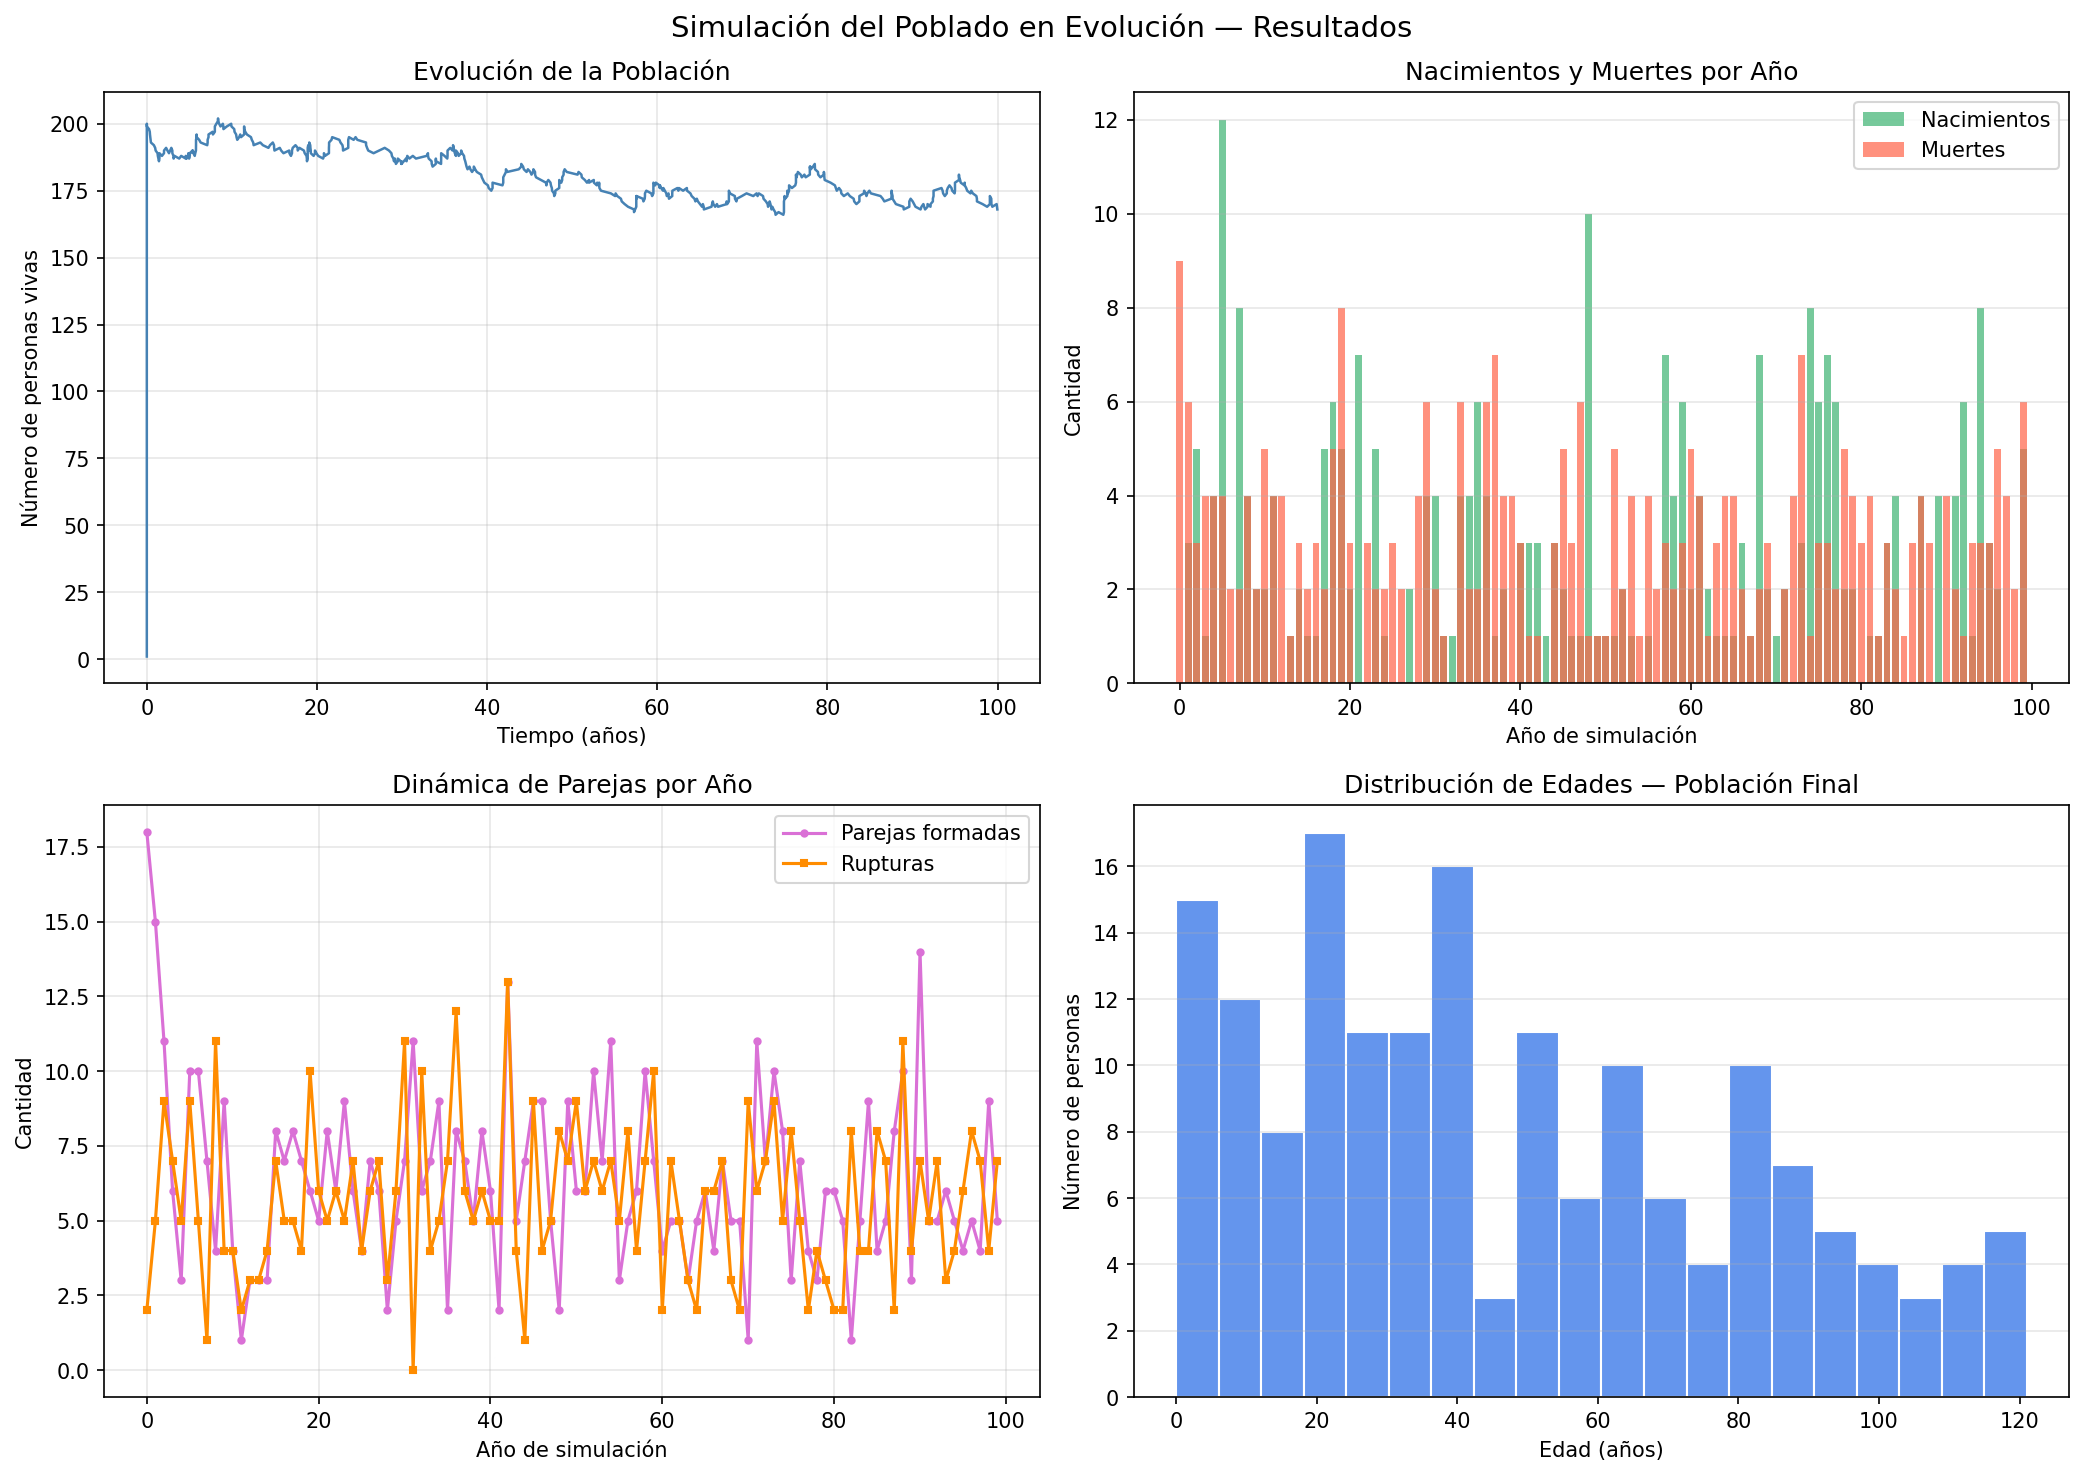
\includegraphics[width=\linewidth]{figures/single_h100_m100.png}
  \caption{Corrida individual (semilla 42): $H=100$, $M=100$, 100 años.}
  \label{fig:single_h100_m100}
\end{figure}

\begin{figure}[H]
  \centering
  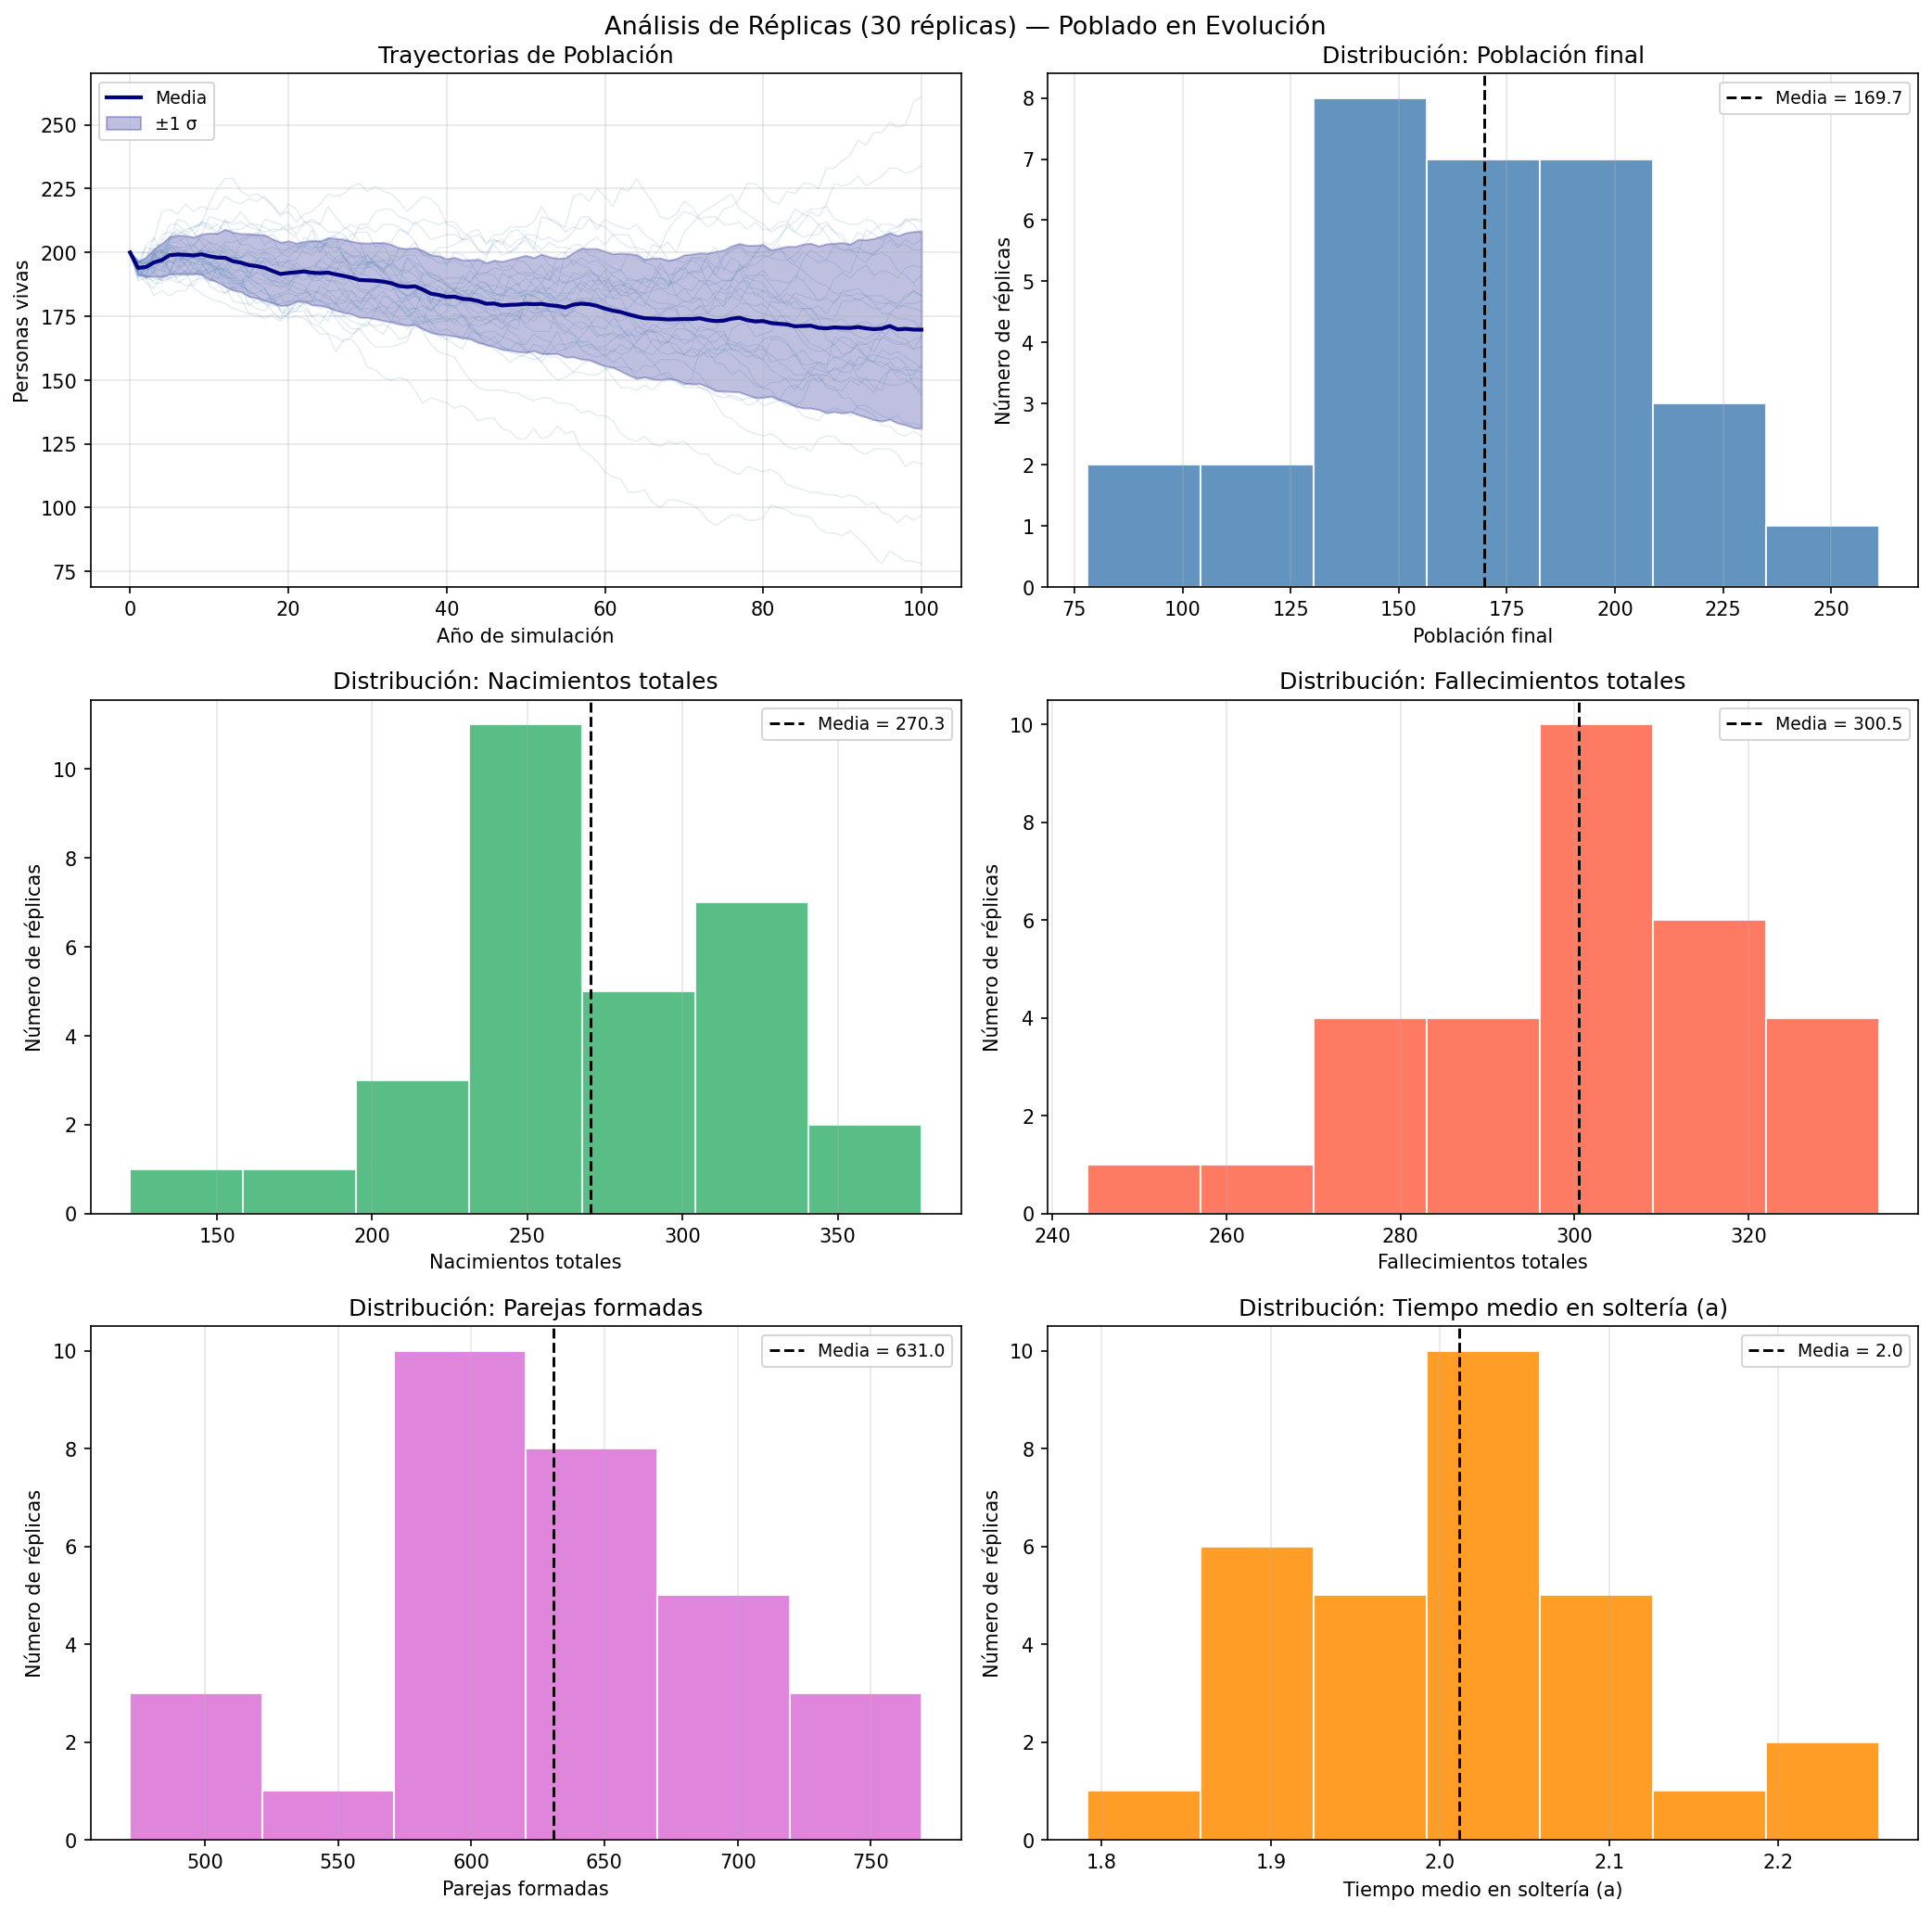
\includegraphics[width=\linewidth]{figures/batch_h100_m100.png}
  \caption{Análisis de 30 réplicas: $H=100$, $M=100$, 100 años.}
  \label{fig:batch_h100_m100}
\end{figure}

% ----------------------------------------------------------------------------
\subsection*{A.2 Variación de $H$ con $M=100$ fijo}
% ----------------------------------------------------------------------------

\begin{figure}[H]
  \centering
  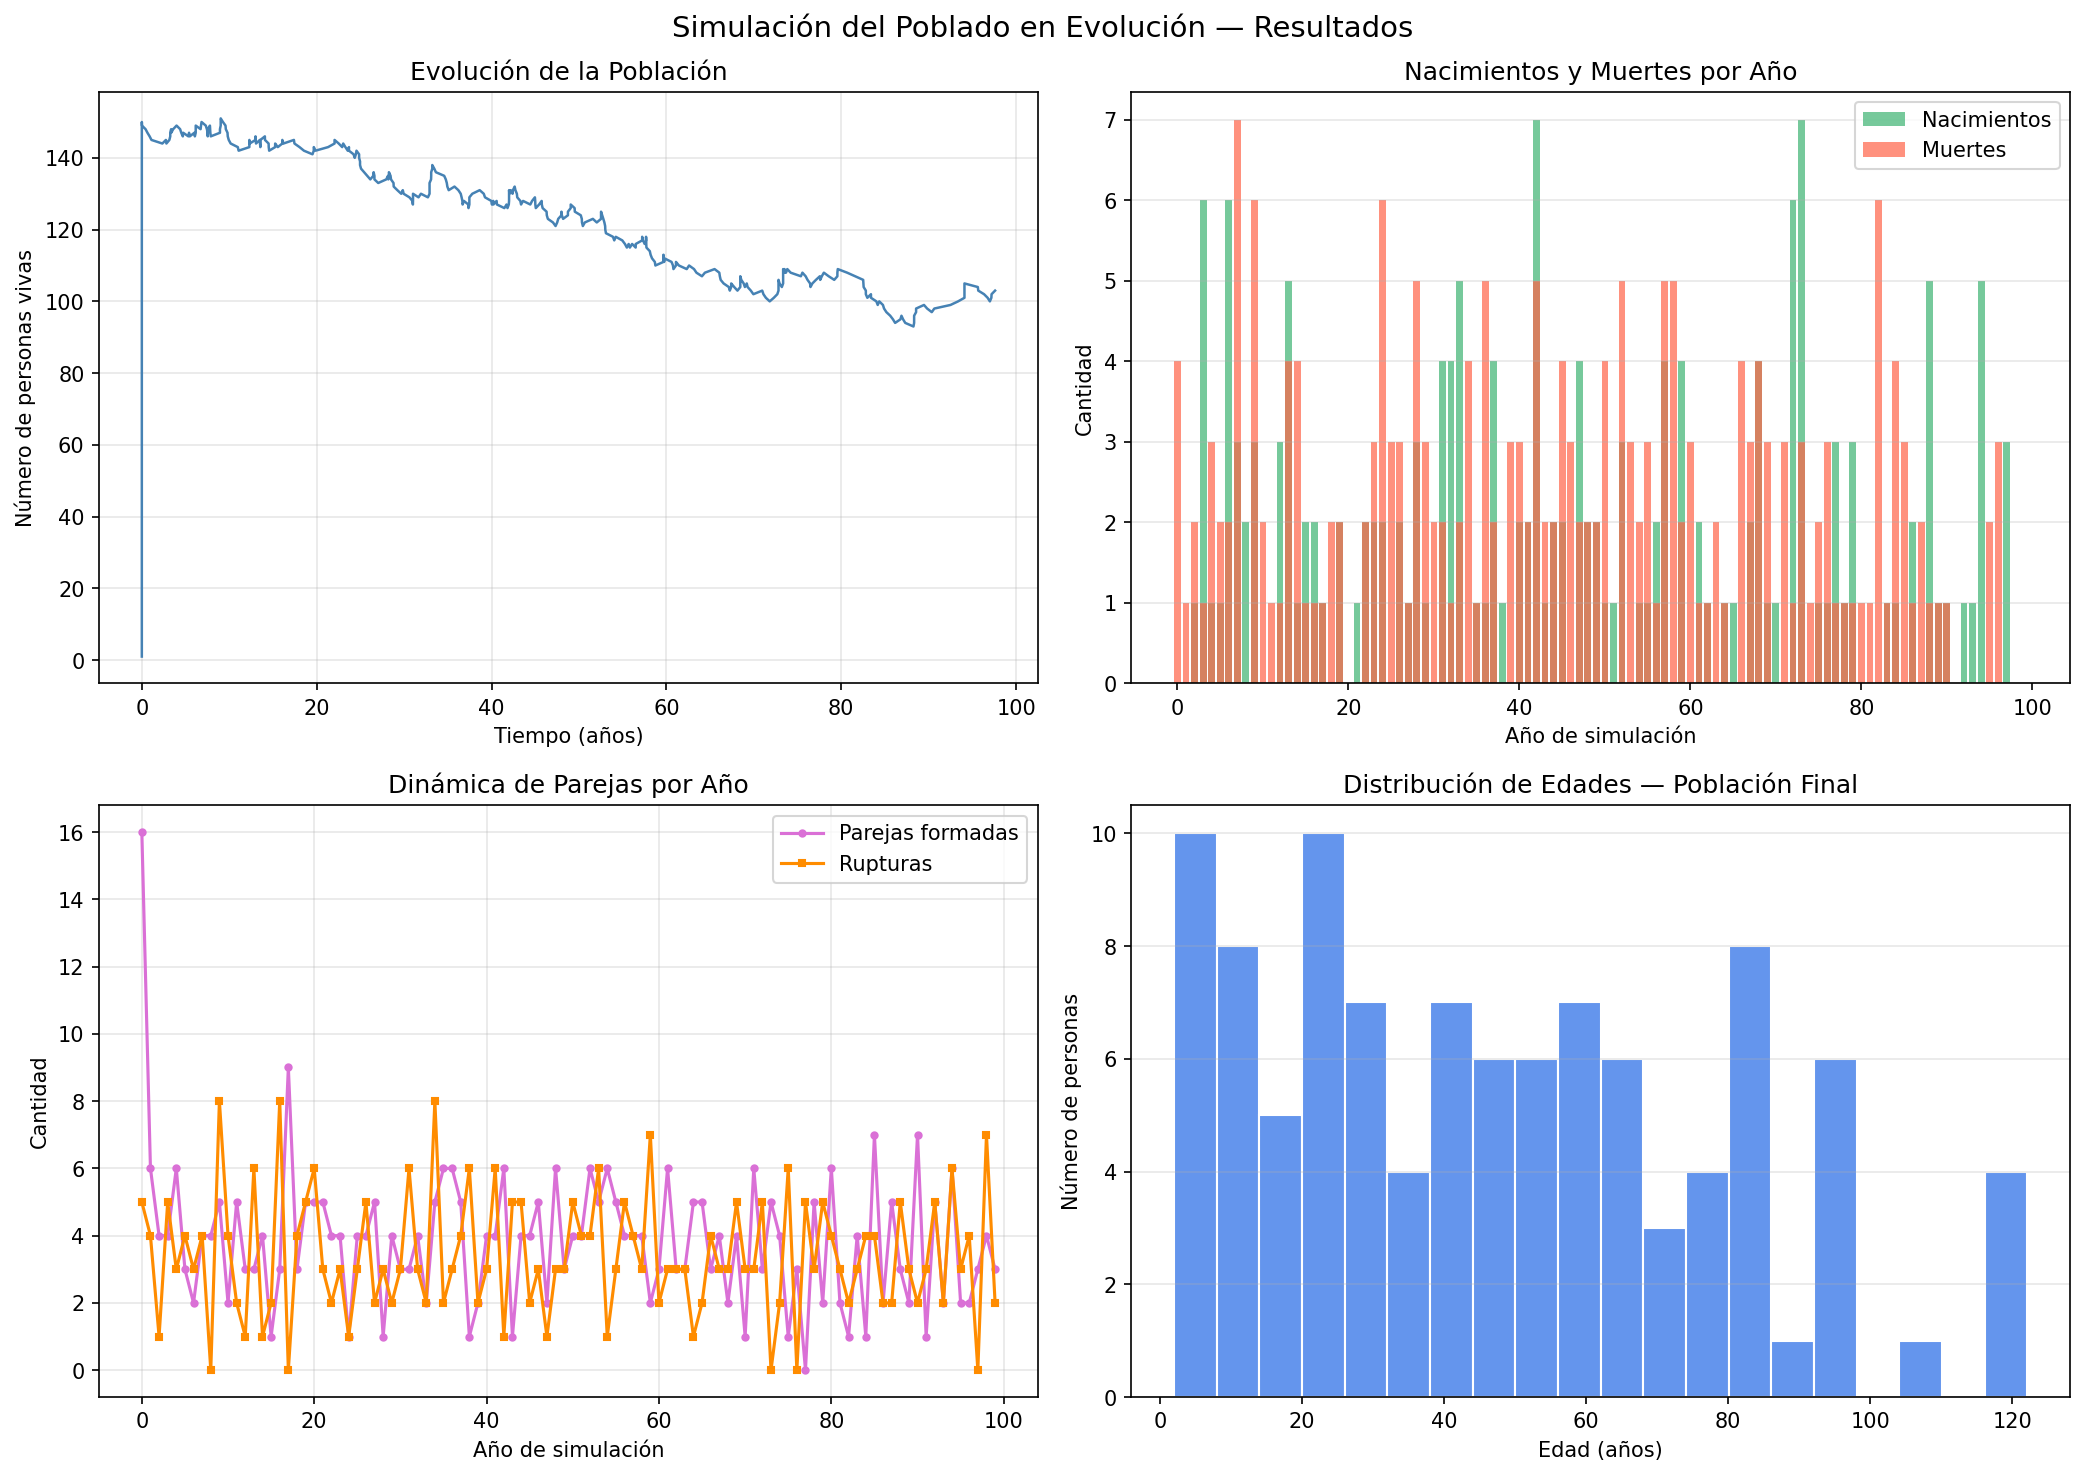
\includegraphics[width=\linewidth]{figures/single_h050_m100.png}
  \caption{Corrida individual (semilla 42): $H=50$, $M=100$.}
  \label{fig:single_h050_m100}
\end{figure}

\begin{figure}[H]
  \centering
  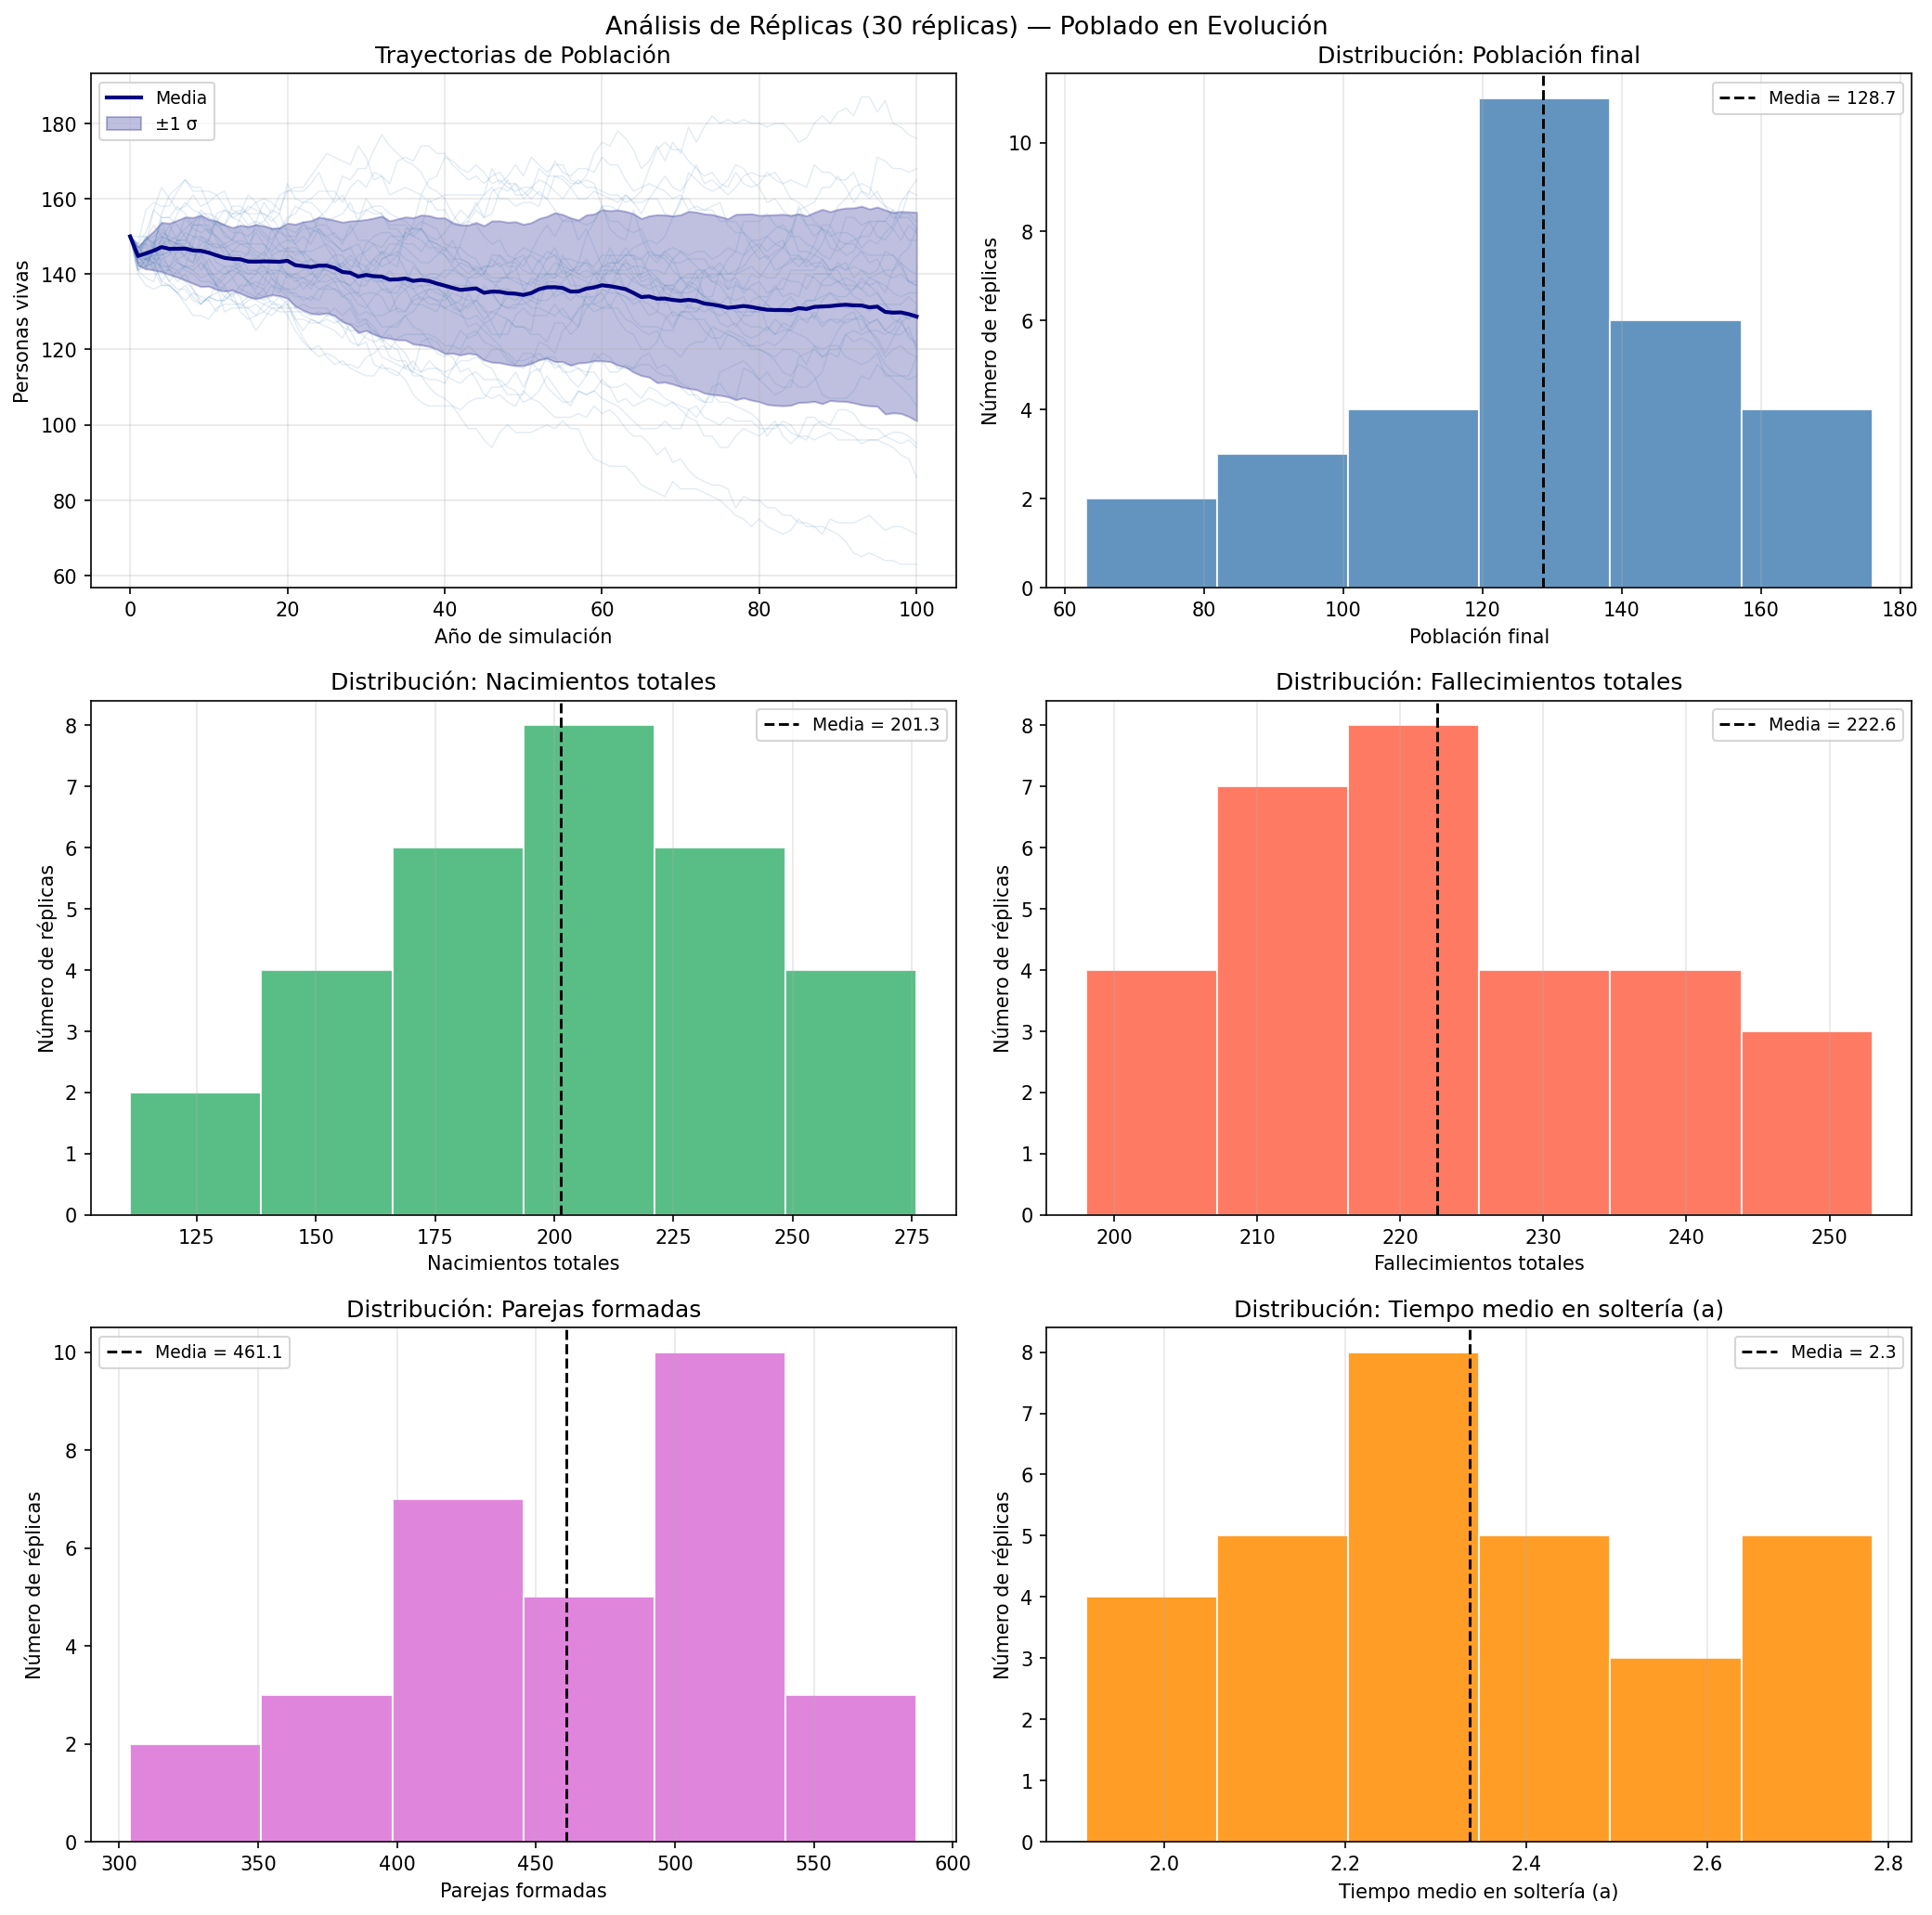
\includegraphics[width=\linewidth]{figures/batch_h050_m100.png}
  \caption{Análisis de 30 réplicas: $H=50$, $M=100$.}
  \label{fig:batch_h050_m100}
\end{figure}

\begin{figure}[H]
  \centering
  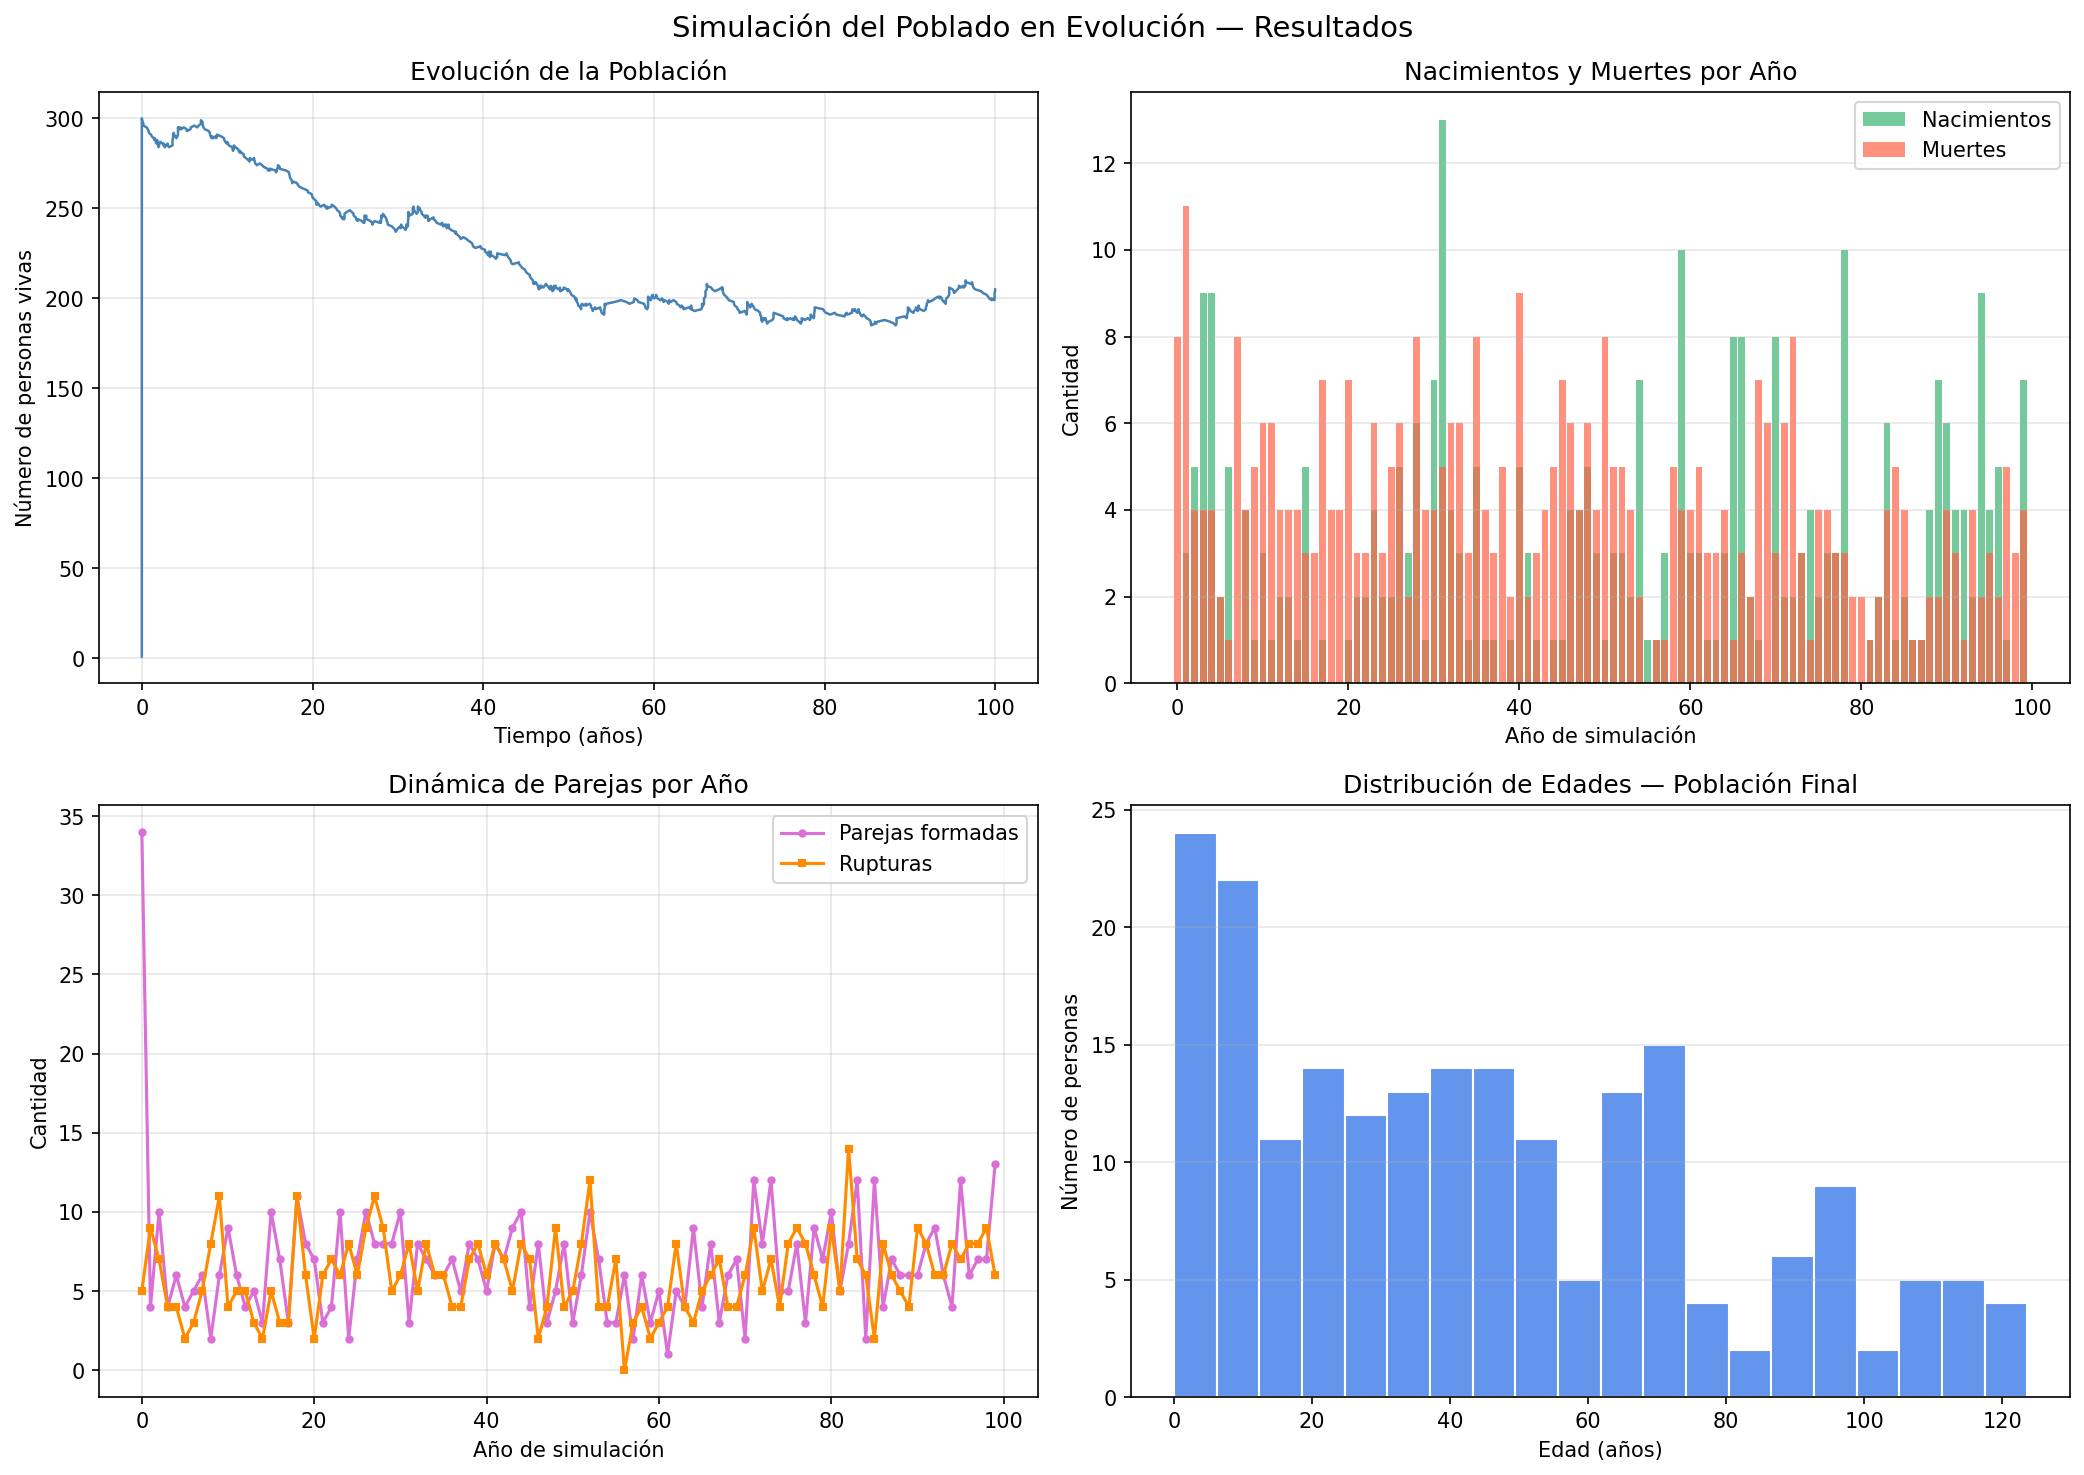
\includegraphics[width=\linewidth]{figures/single_h200_m100.png}
  \caption{Corrida individual (semilla 42): $H=200$, $M=100$.}
  \label{fig:single_h200_m100}
\end{figure}

\begin{figure}[H]
  \centering
  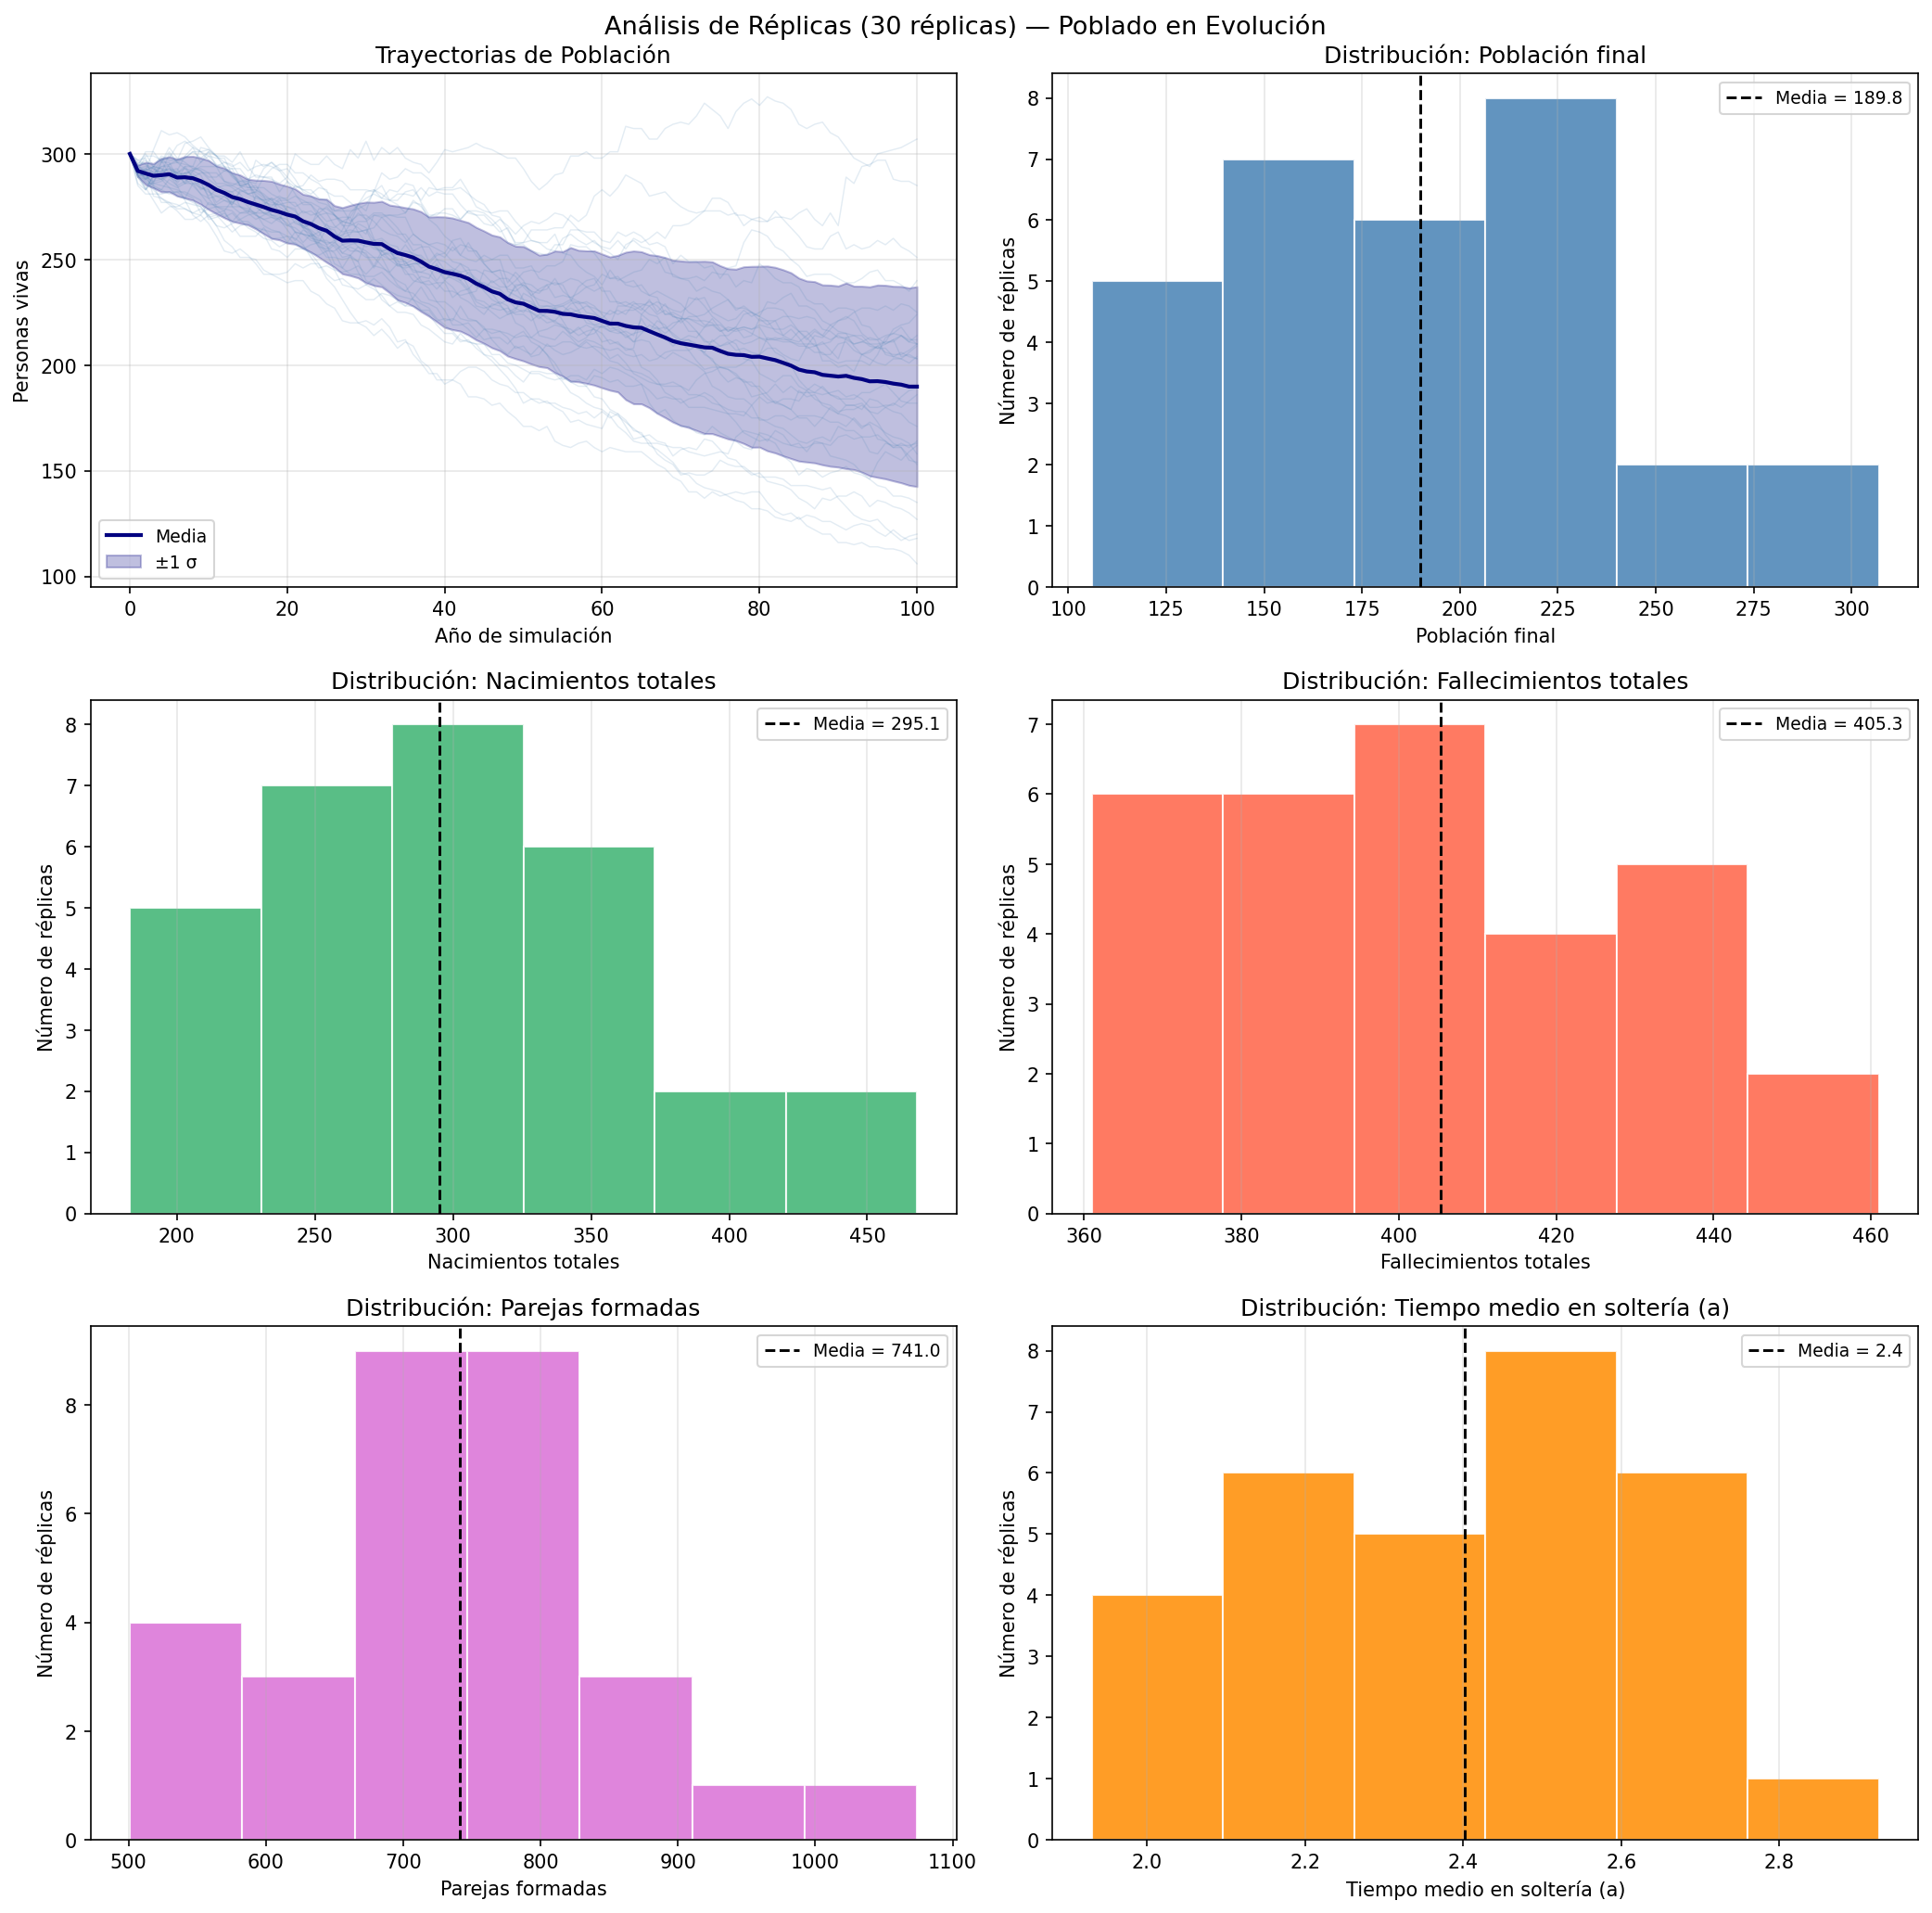
\includegraphics[width=\linewidth]{figures/batch_h200_m100.png}
  \caption{Análisis de 30 réplicas: $H=200$, $M=100$.}
  \label{fig:batch_h200_m100}
\end{figure}

\begin{figure}[H]
  \centering
  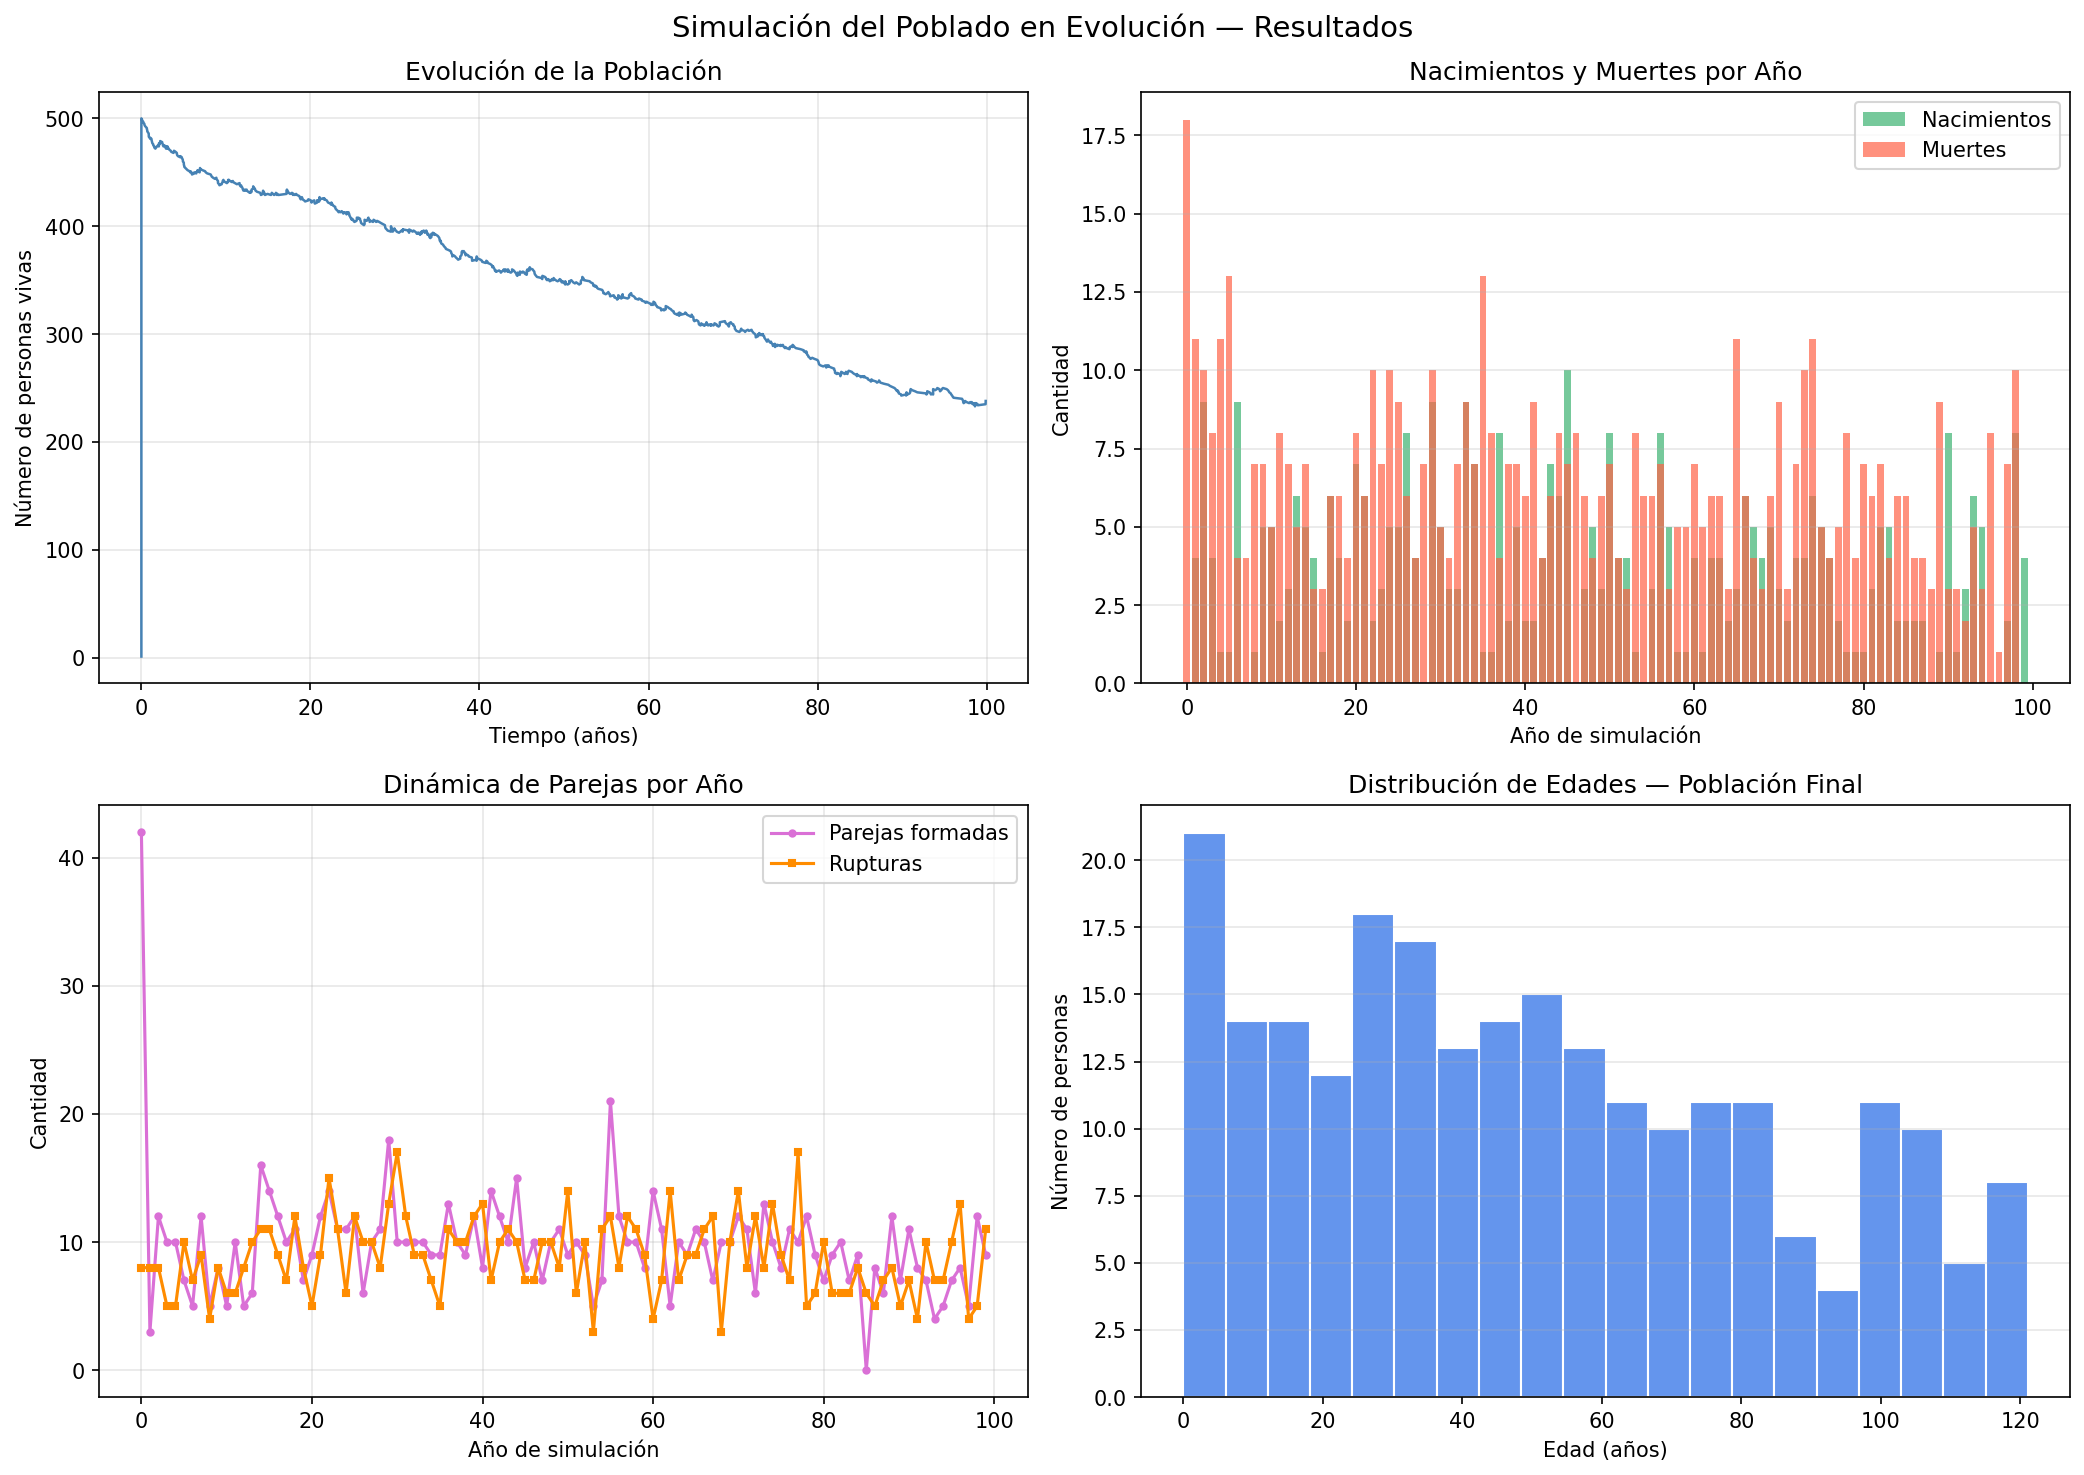
\includegraphics[width=\linewidth]{figures/single_h400_m100.png}
  \caption{Corrida individual (semilla 42): $H=400$, $M=100$.}
  \label{fig:single_h400_m100}
\end{figure}

\begin{figure}[H]
  \centering
  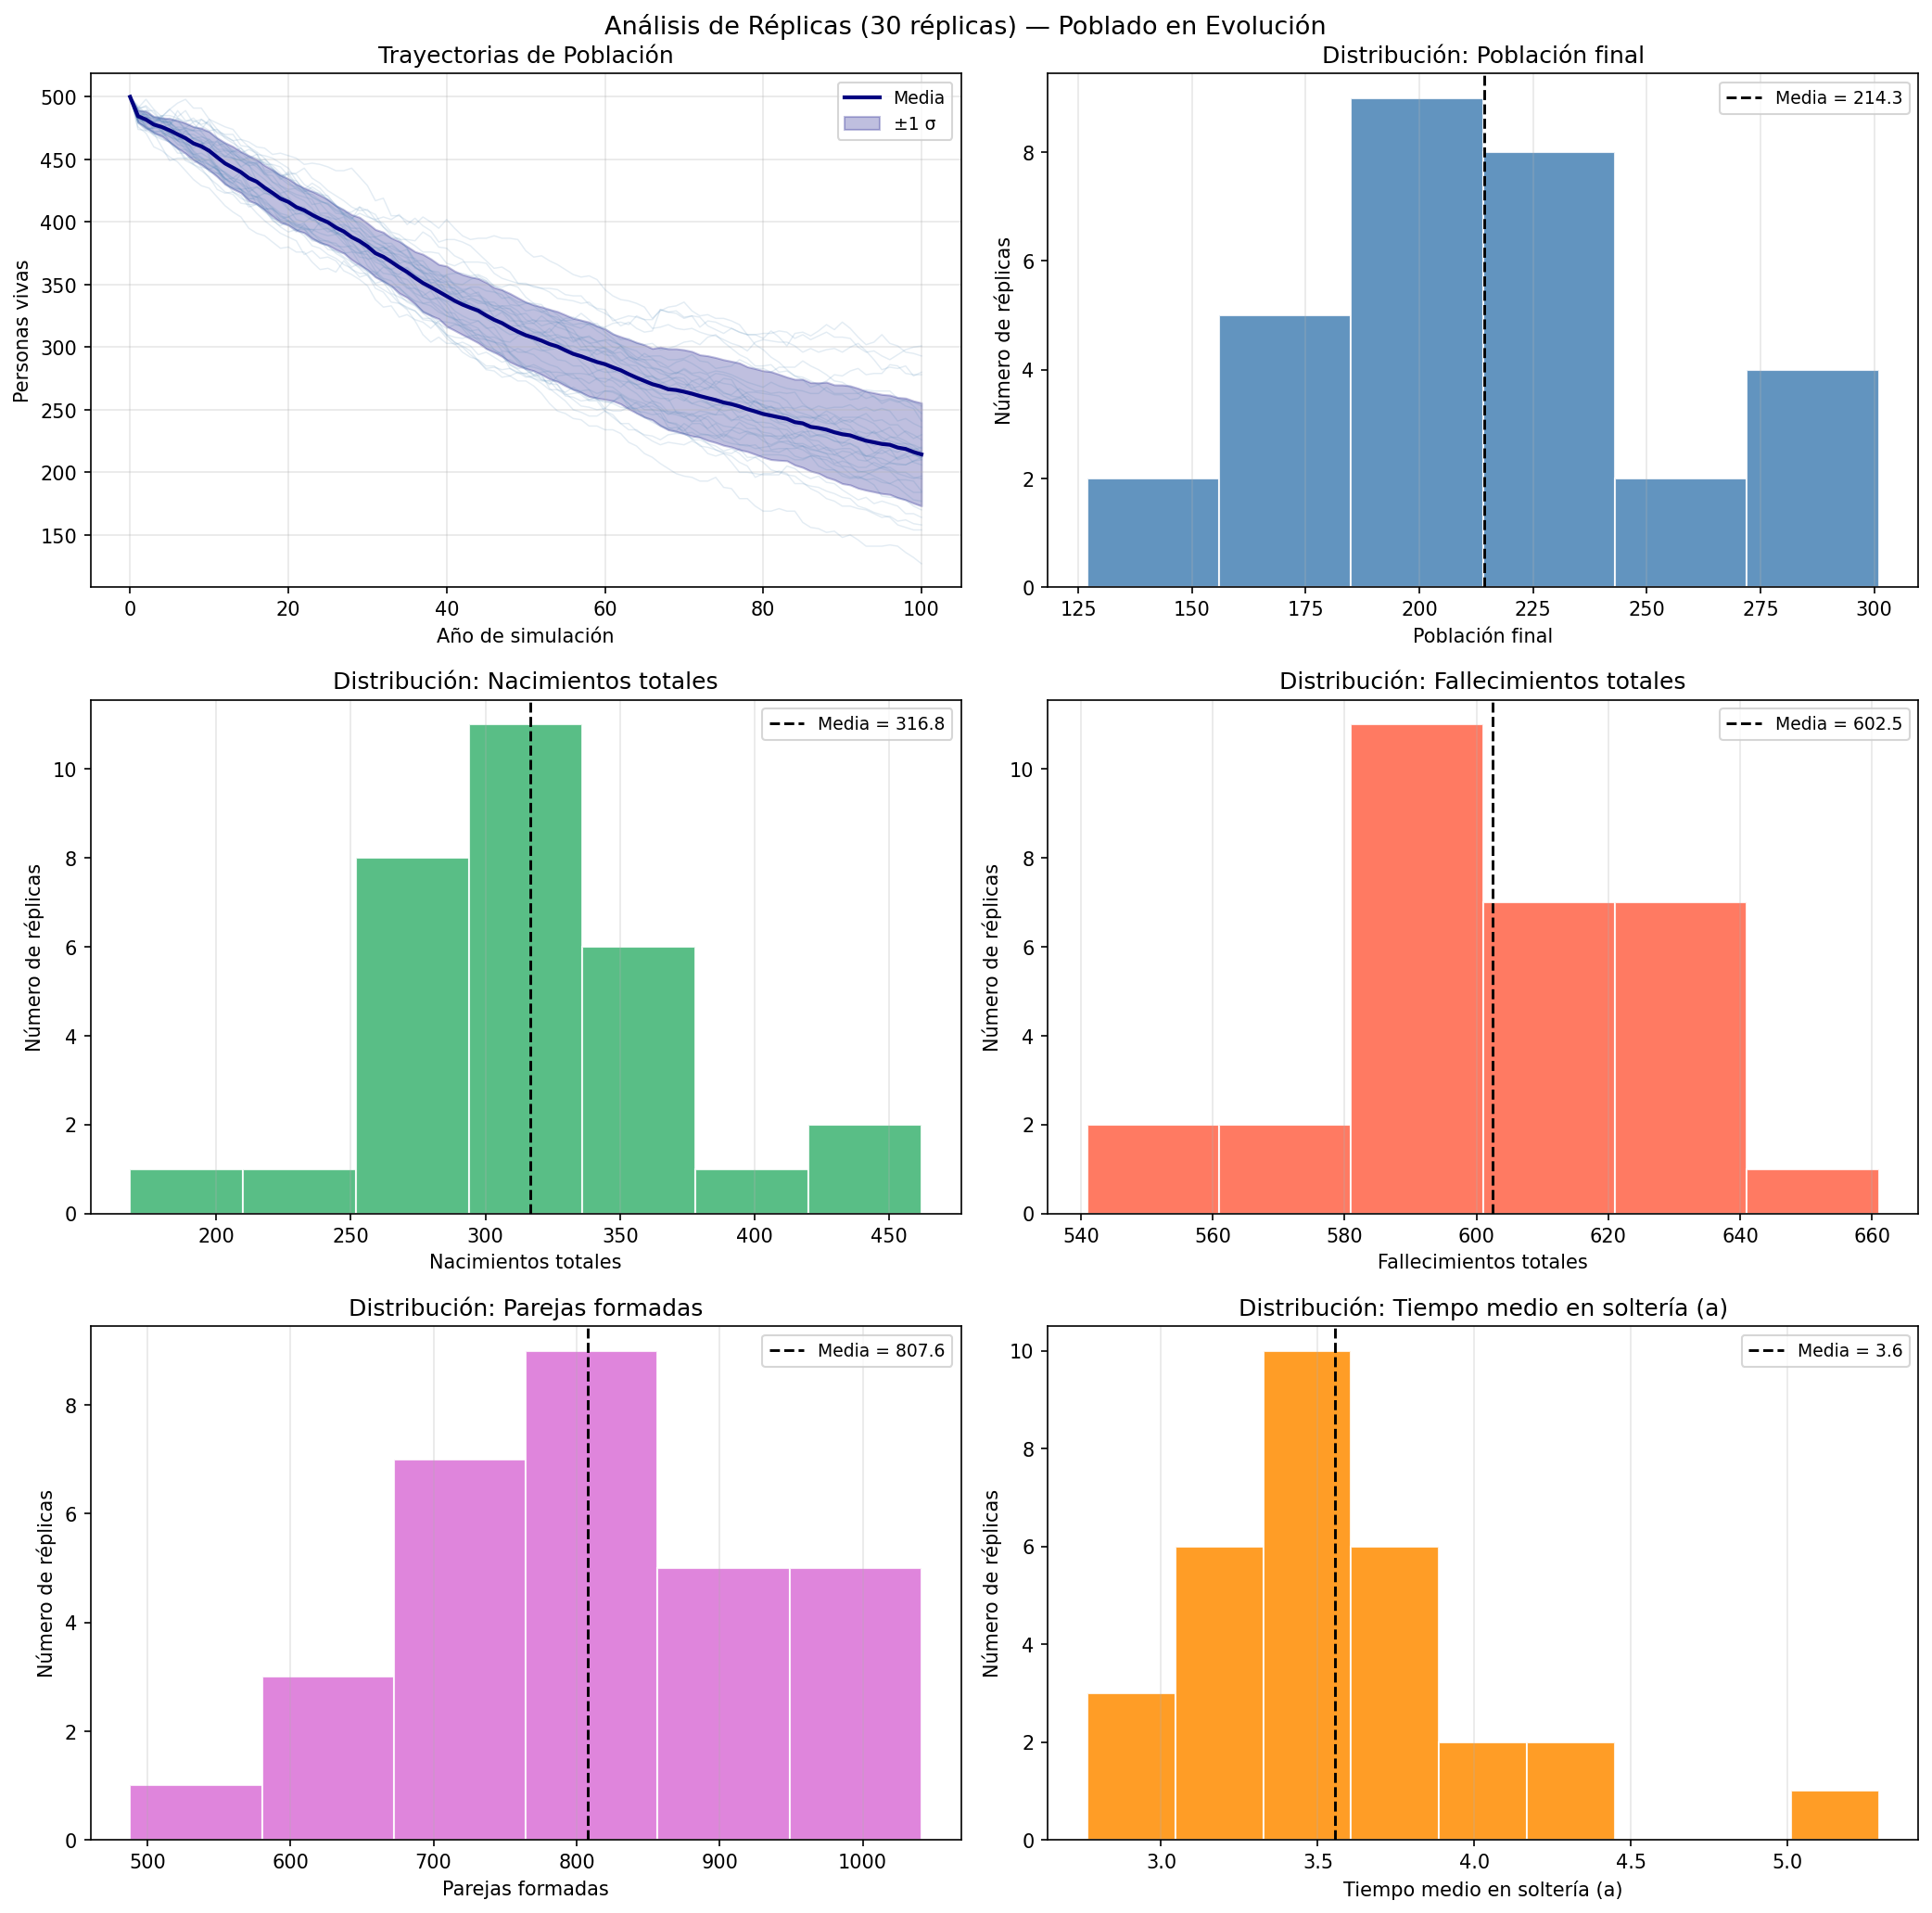
\includegraphics[width=\linewidth]{figures/batch_h400_m100.png}
  \caption{Análisis de 30 réplicas: $H=400$, $M=100$.}
  \label{fig:batch_h400_m100}
\end{figure}

% ----------------------------------------------------------------------------
\subsection*{A.3 Variación de $M$ con $H=100$ fijo}
% ----------------------------------------------------------------------------

\begin{figure}[H]
  \centering
  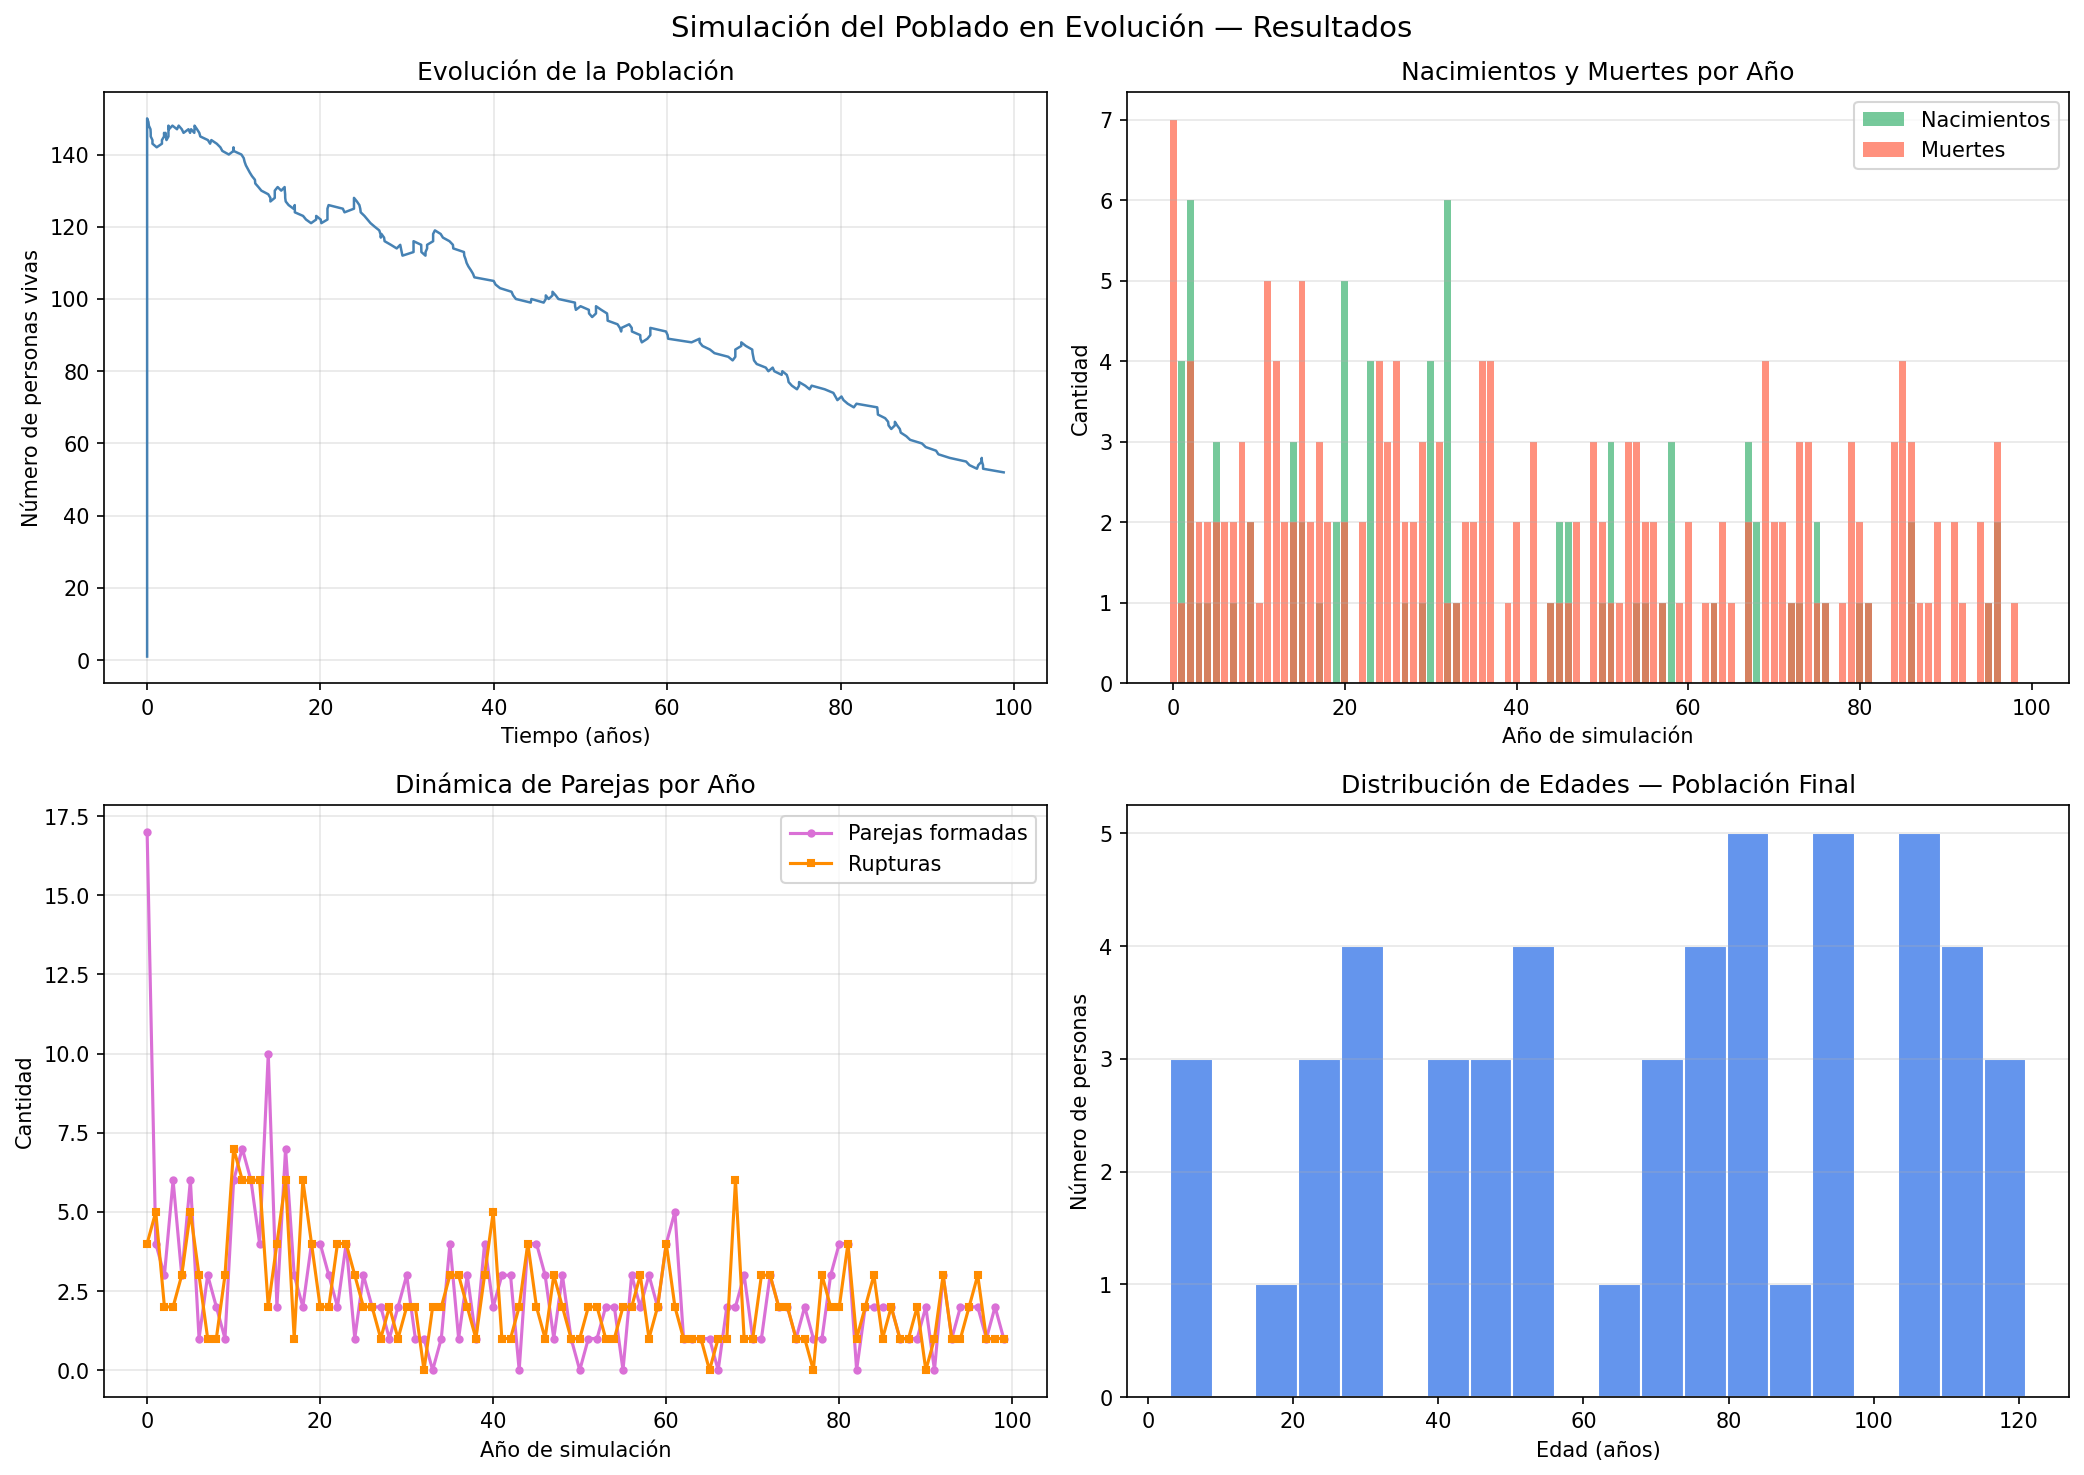
\includegraphics[width=\linewidth]{figures/single_h100_m050.png}
  \caption{Corrida individual (semilla 42): $H=100$, $M=50$.}
  \label{fig:single_h100_m050}
\end{figure}

\begin{figure}[H]
  \centering
  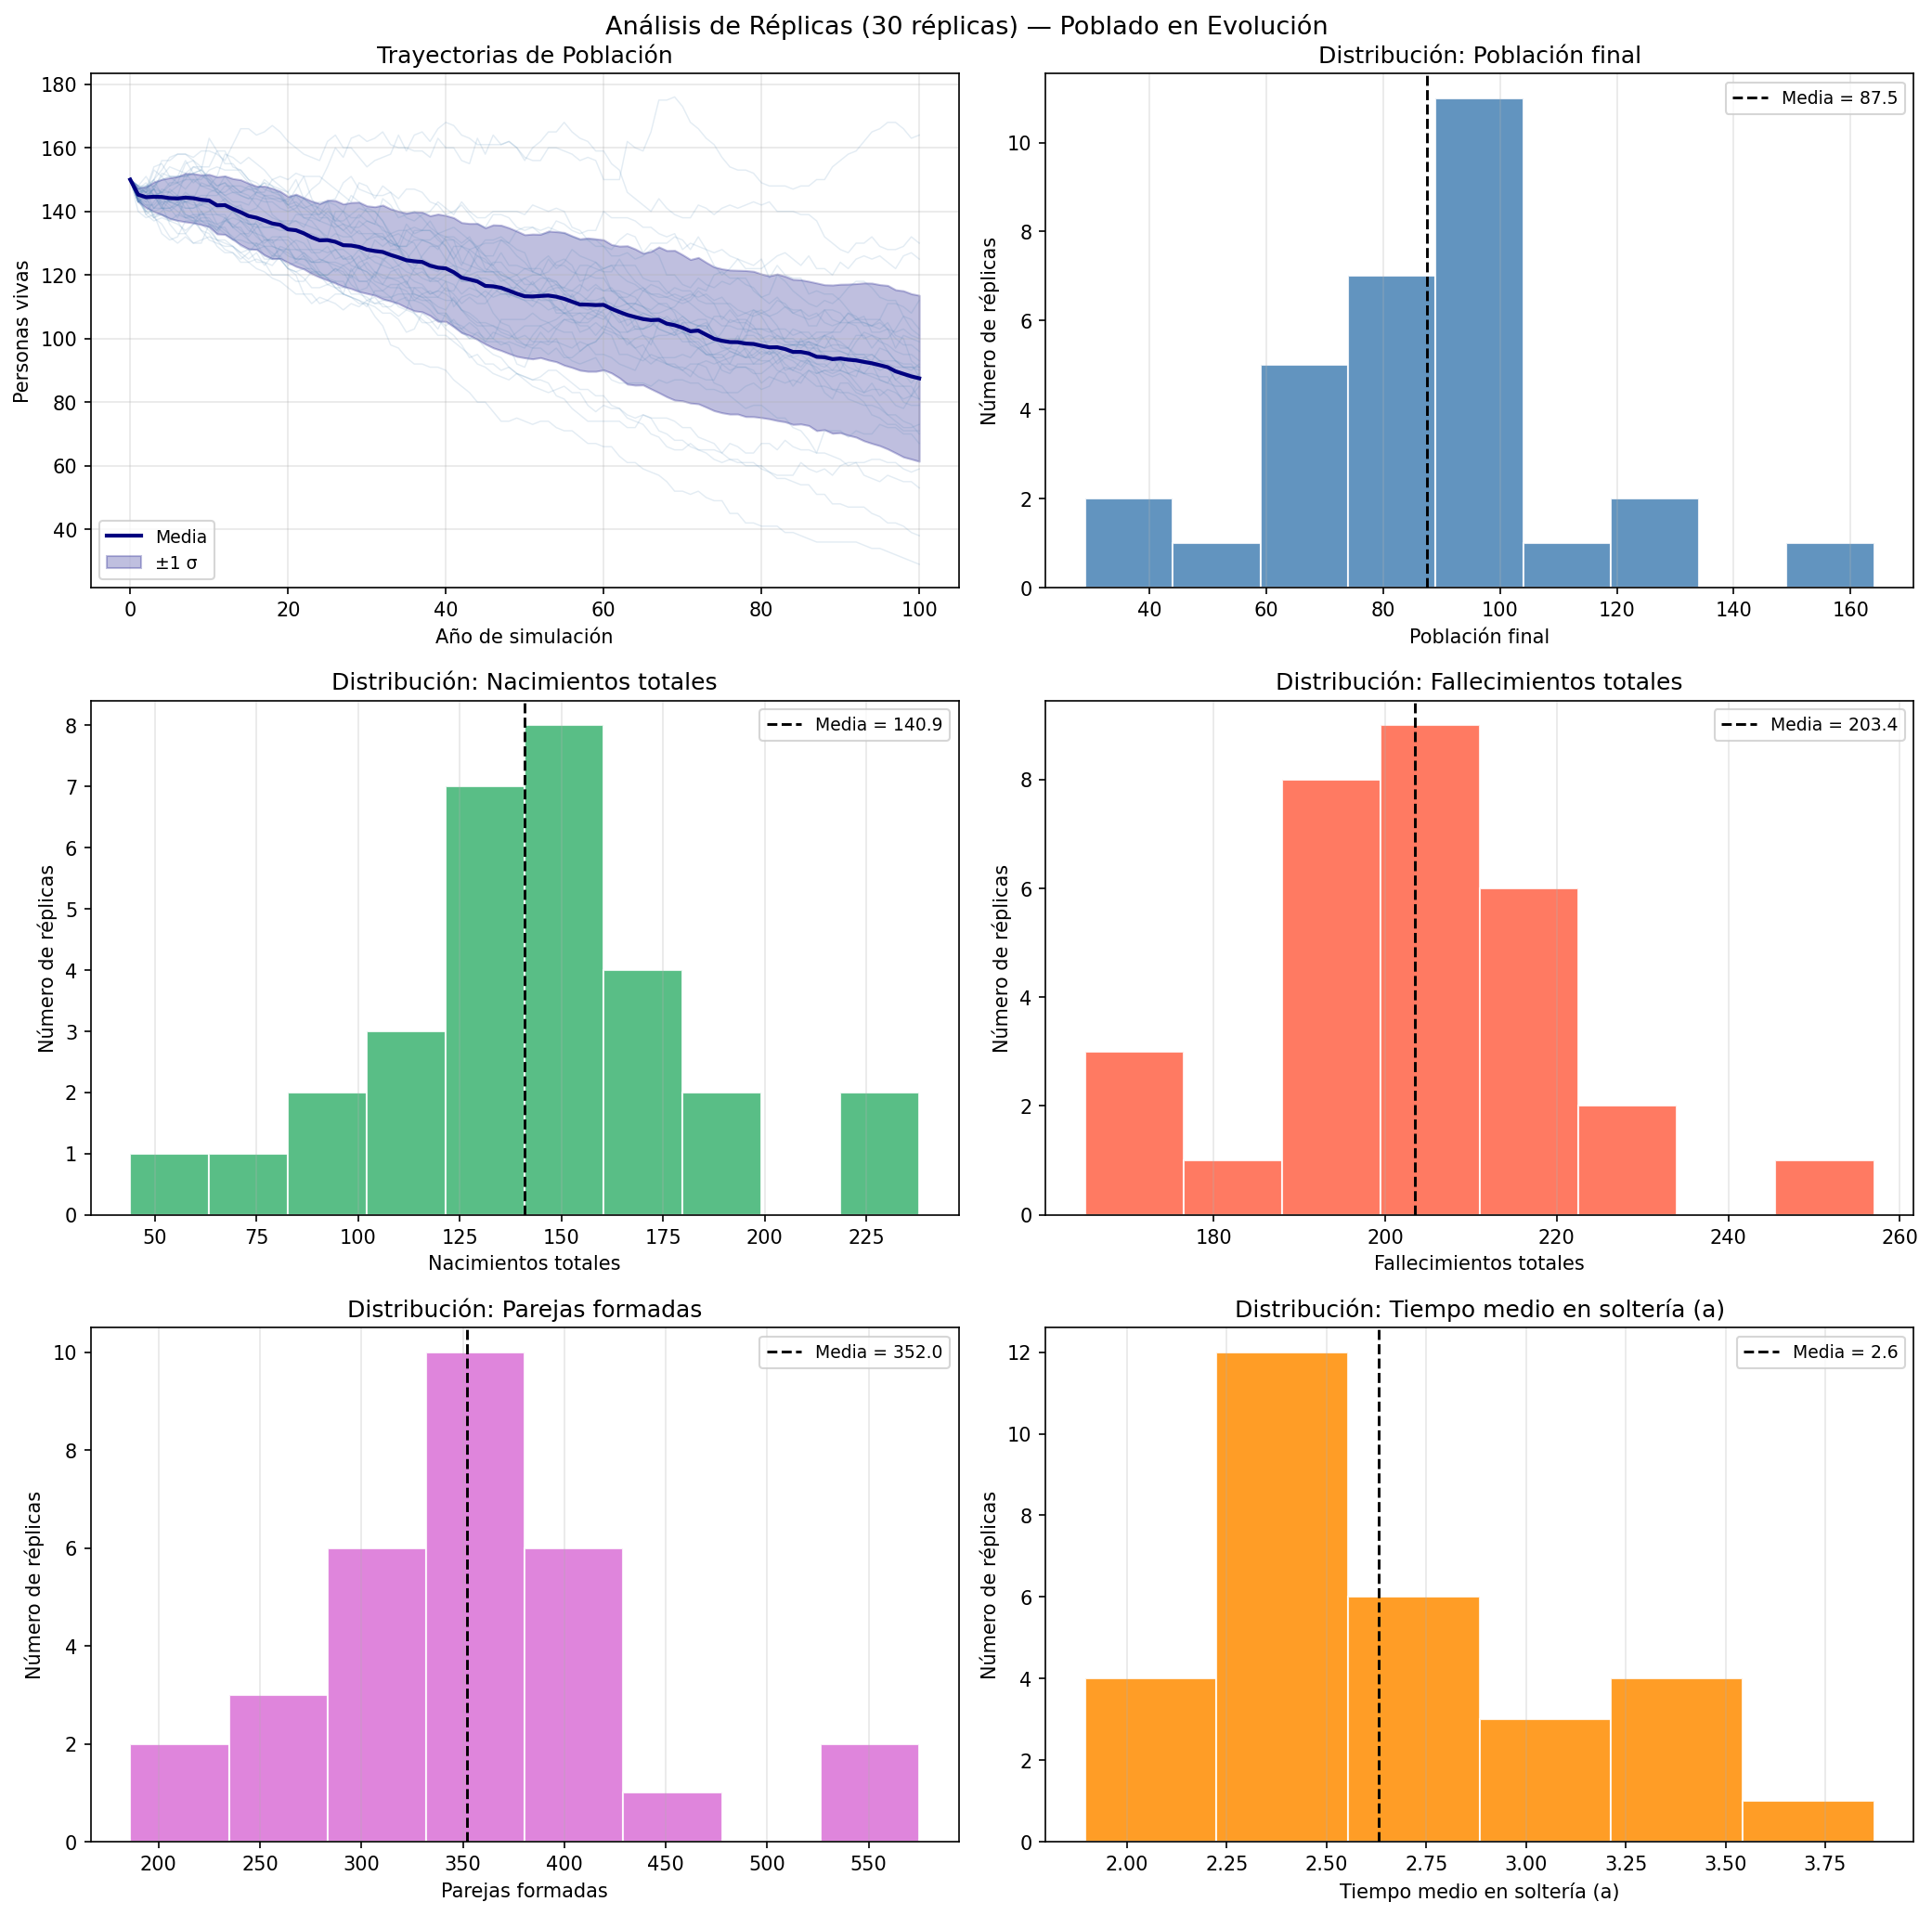
\includegraphics[width=\linewidth]{figures/batch_h100_m050.png}
  \caption{Análisis de 30 réplicas: $H=100$, $M=50$.}
  \label{fig:batch_h100_m050}
\end{figure}

\begin{figure}[H]
  \centering
  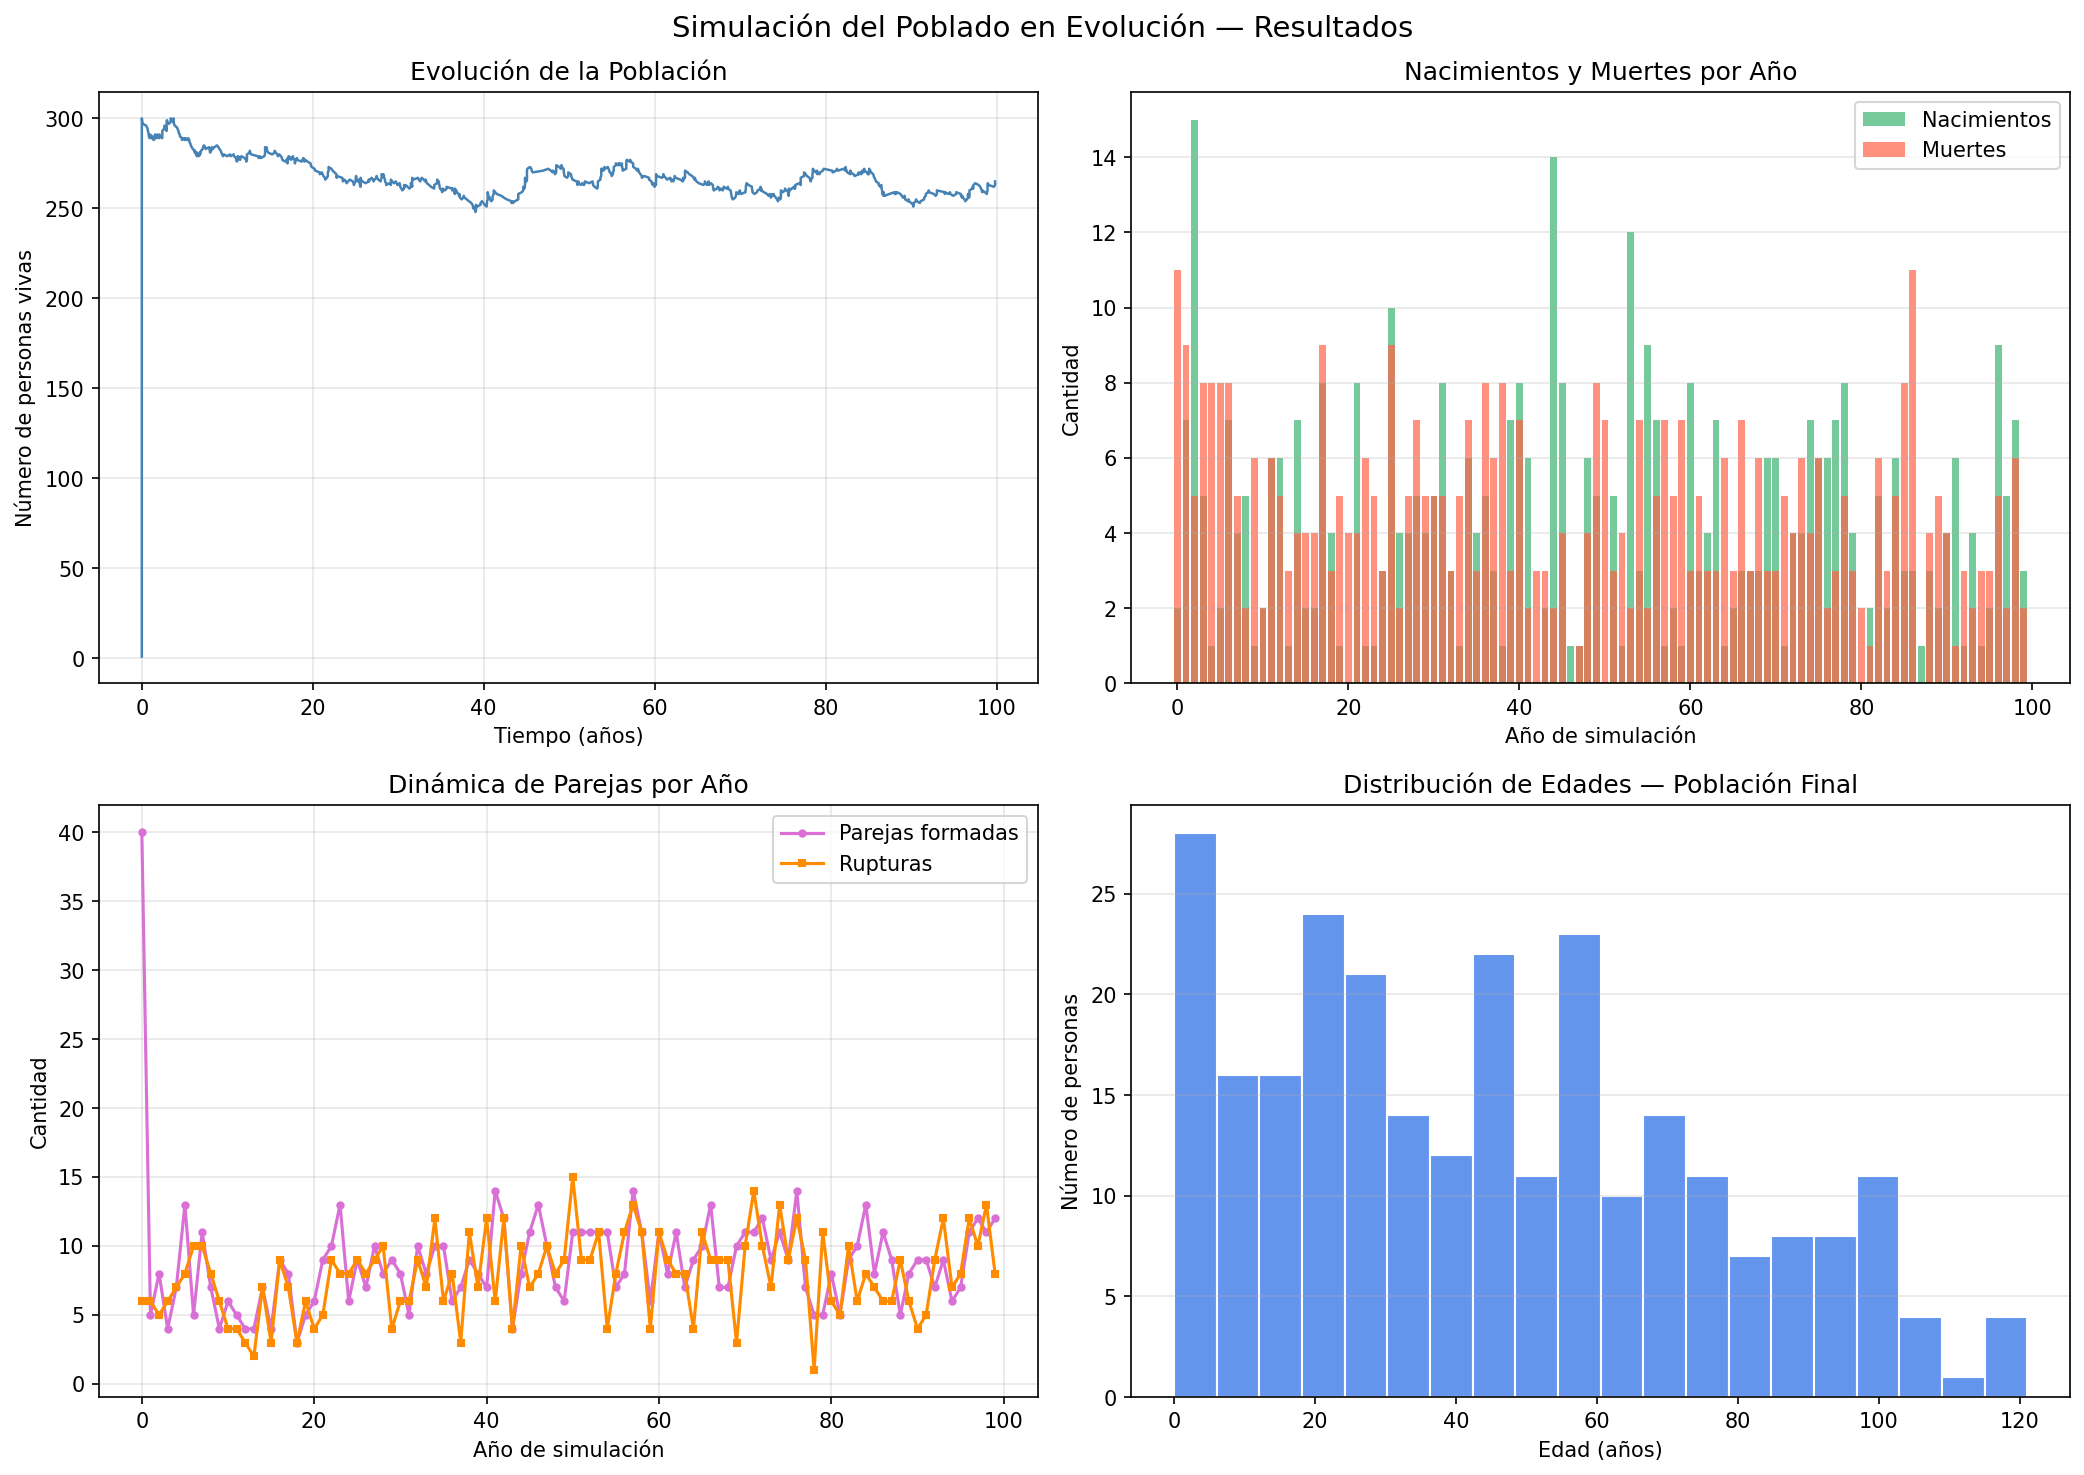
\includegraphics[width=\linewidth]{figures/single_h100_m200.png}
  \caption{Corrida individual (semilla 42): $H=100$, $M=200$.}
  \label{fig:single_h100_m200}
\end{figure}

\begin{figure}[H]
  \centering
  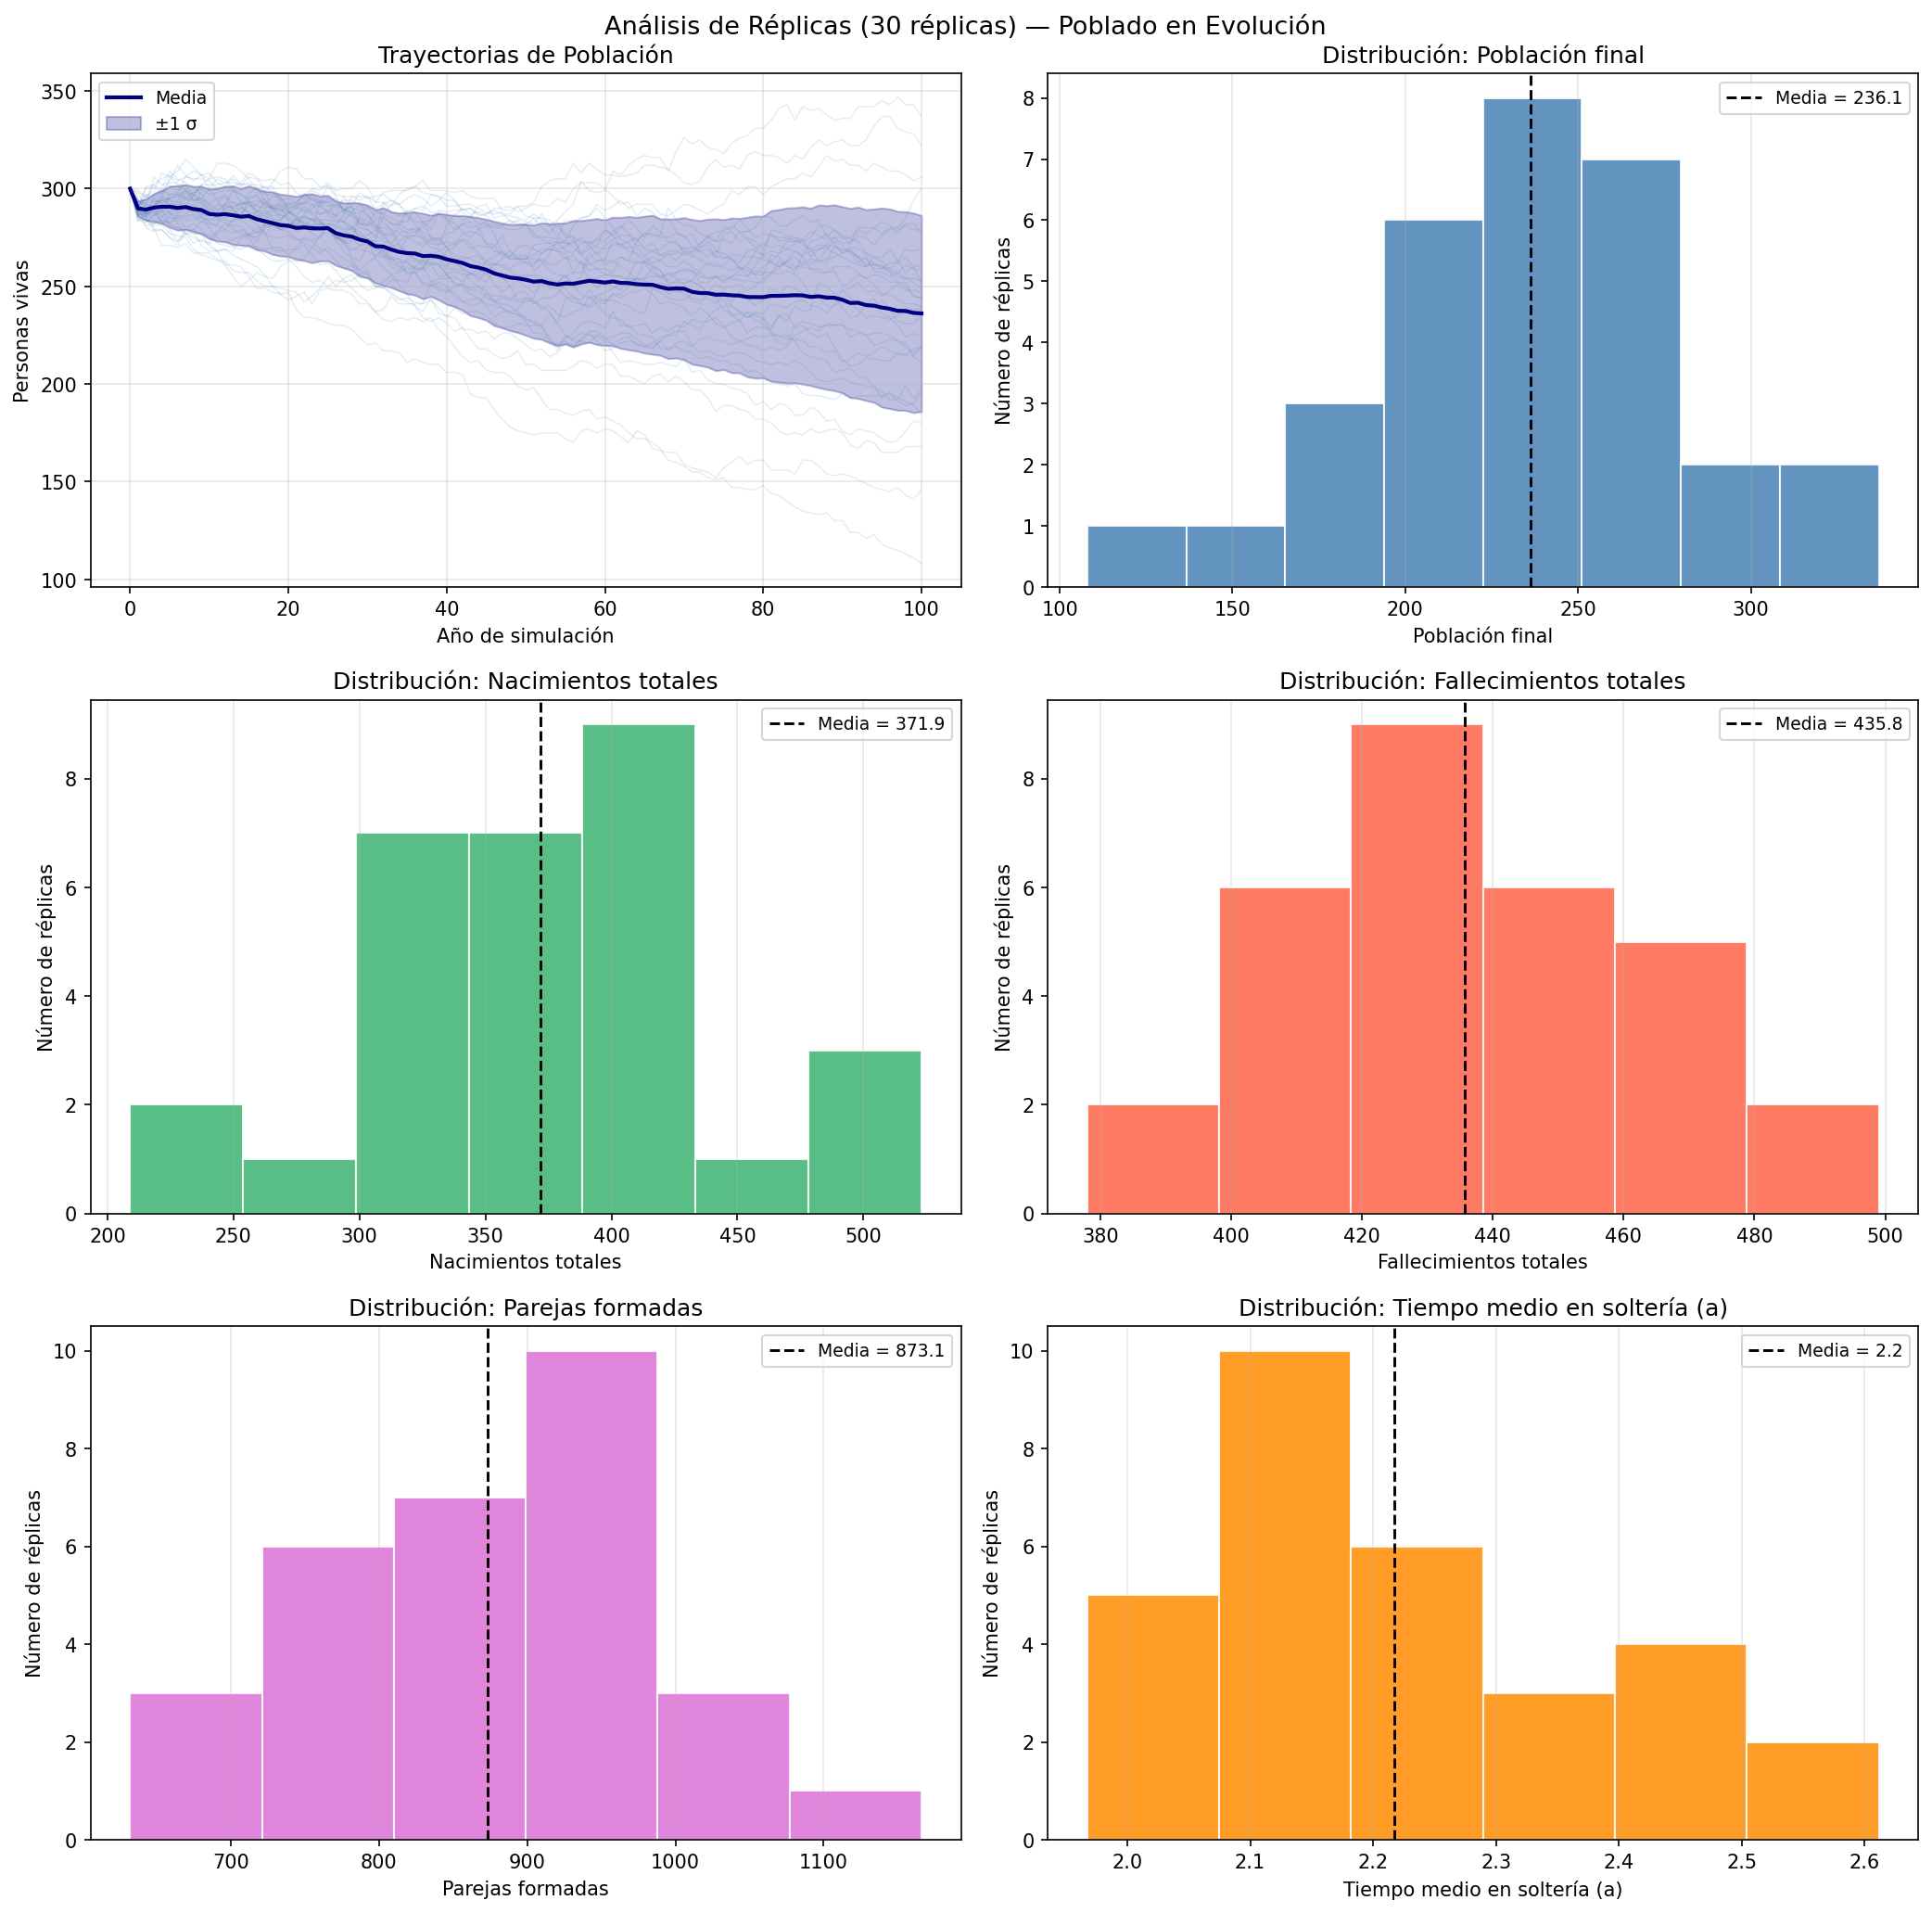
\includegraphics[width=\linewidth]{figures/batch_h100_m200.png}
  \caption{Análisis de 30 réplicas: $H=100$, $M=200$.}
  \label{fig:batch_h100_m200}
\end{figure}

\begin{figure}[H]
  \centering
  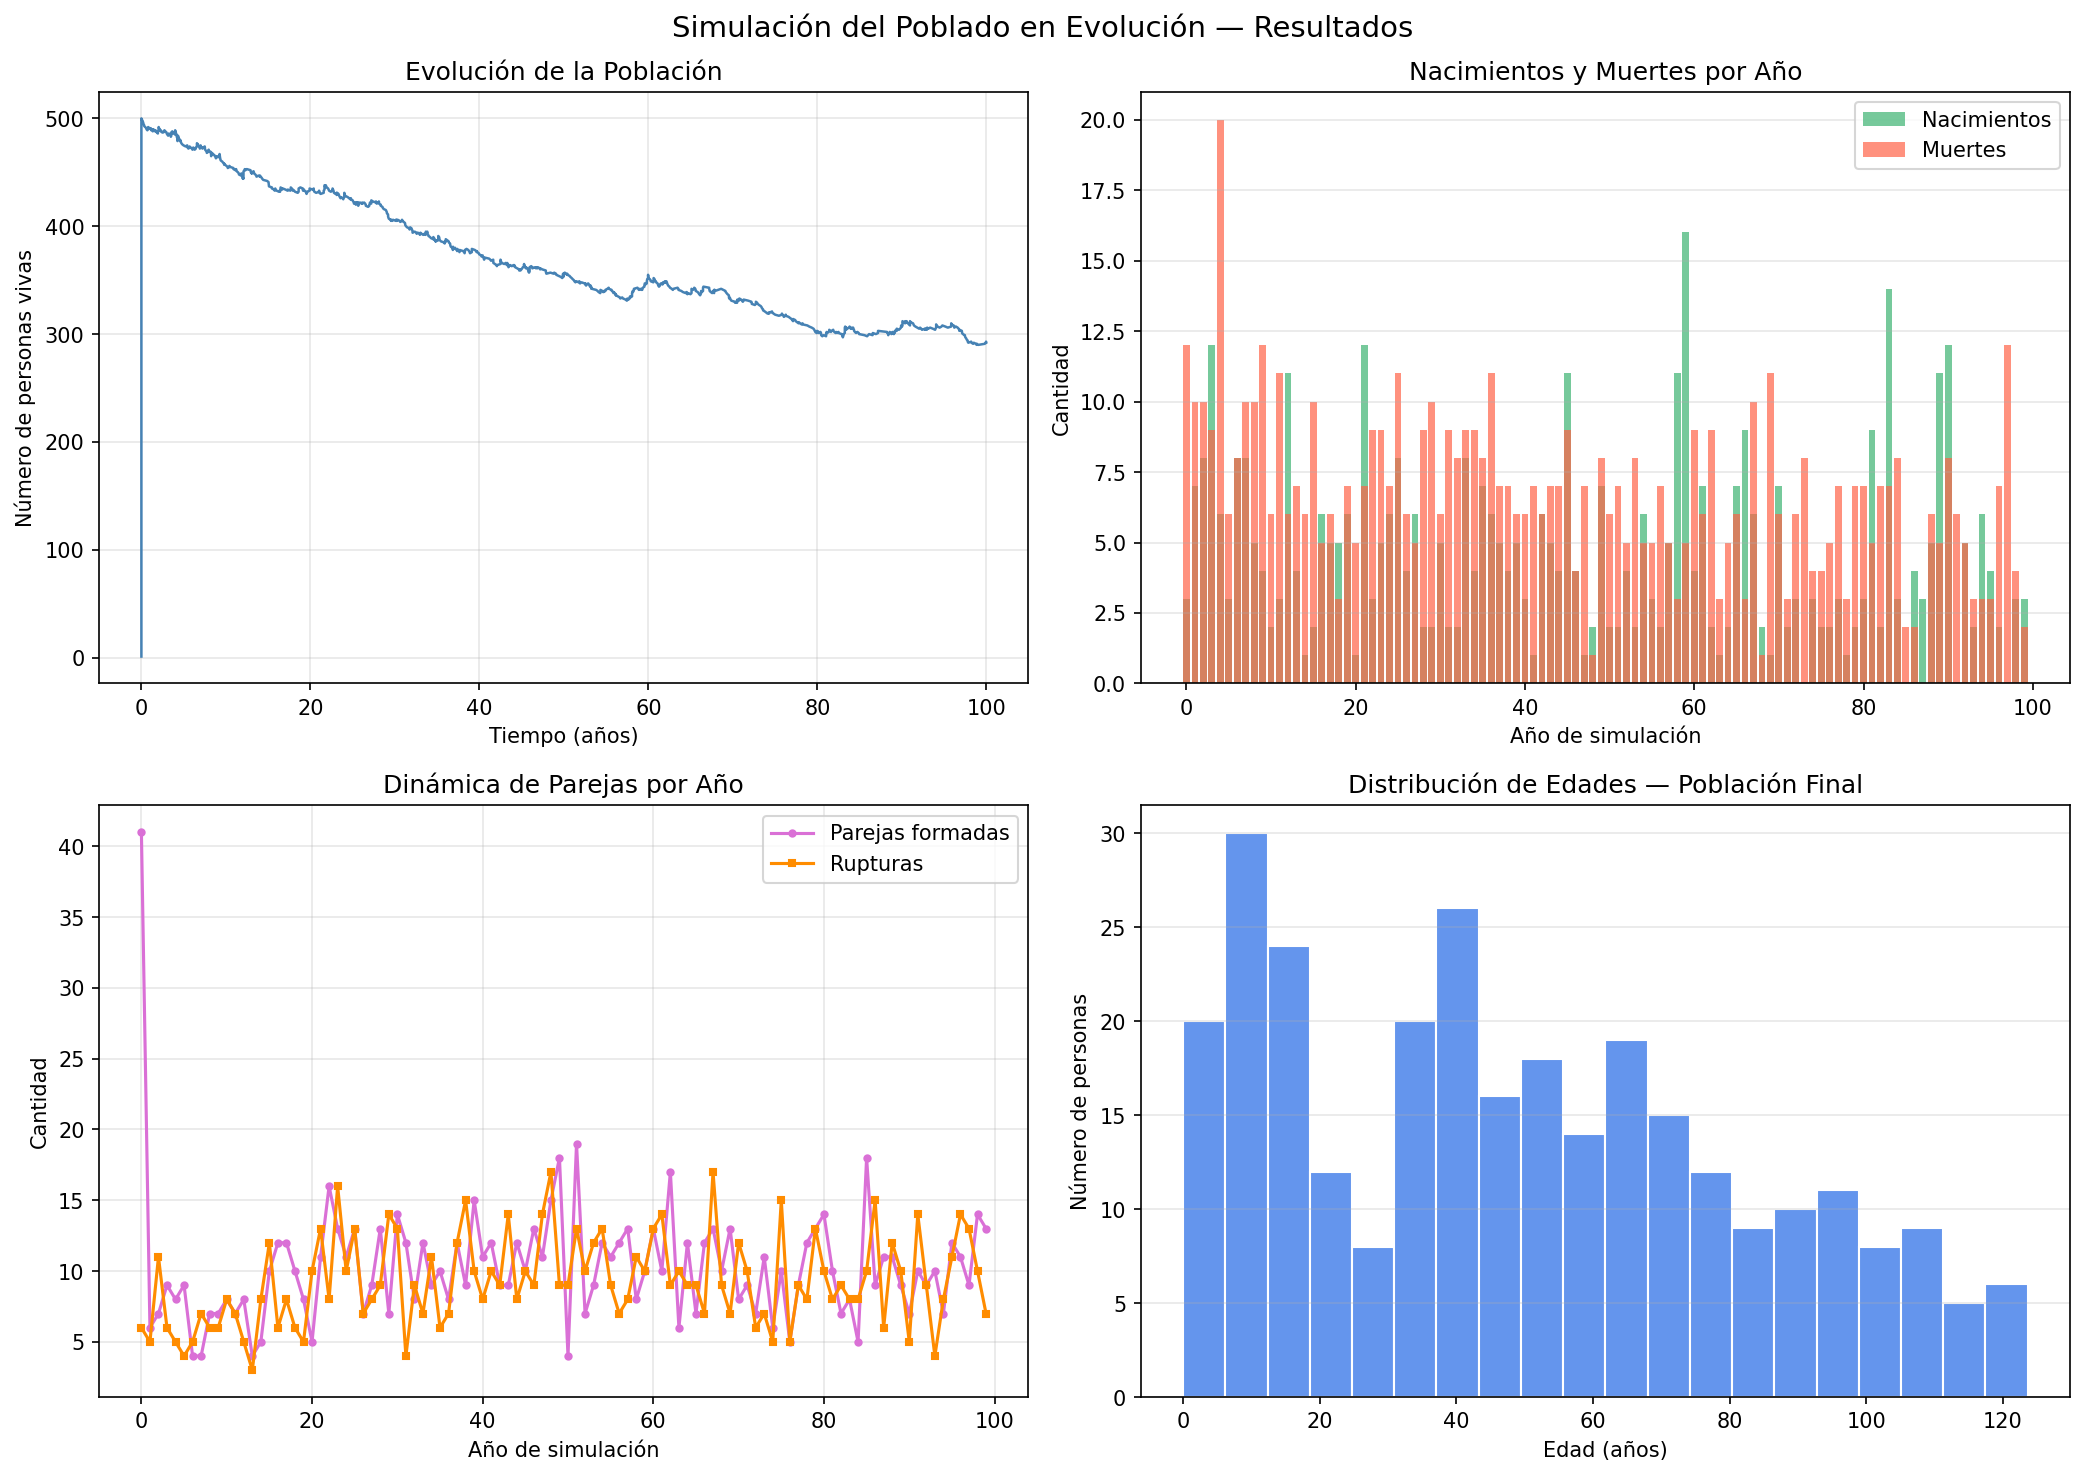
\includegraphics[width=\linewidth]{figures/single_h100_m400.png}
  \caption{Corrida individual (semilla 42): $H=100$, $M=400$.}
  \label{fig:single_h100_m400}
\end{figure}

\begin{figure}[H]
  \centering
  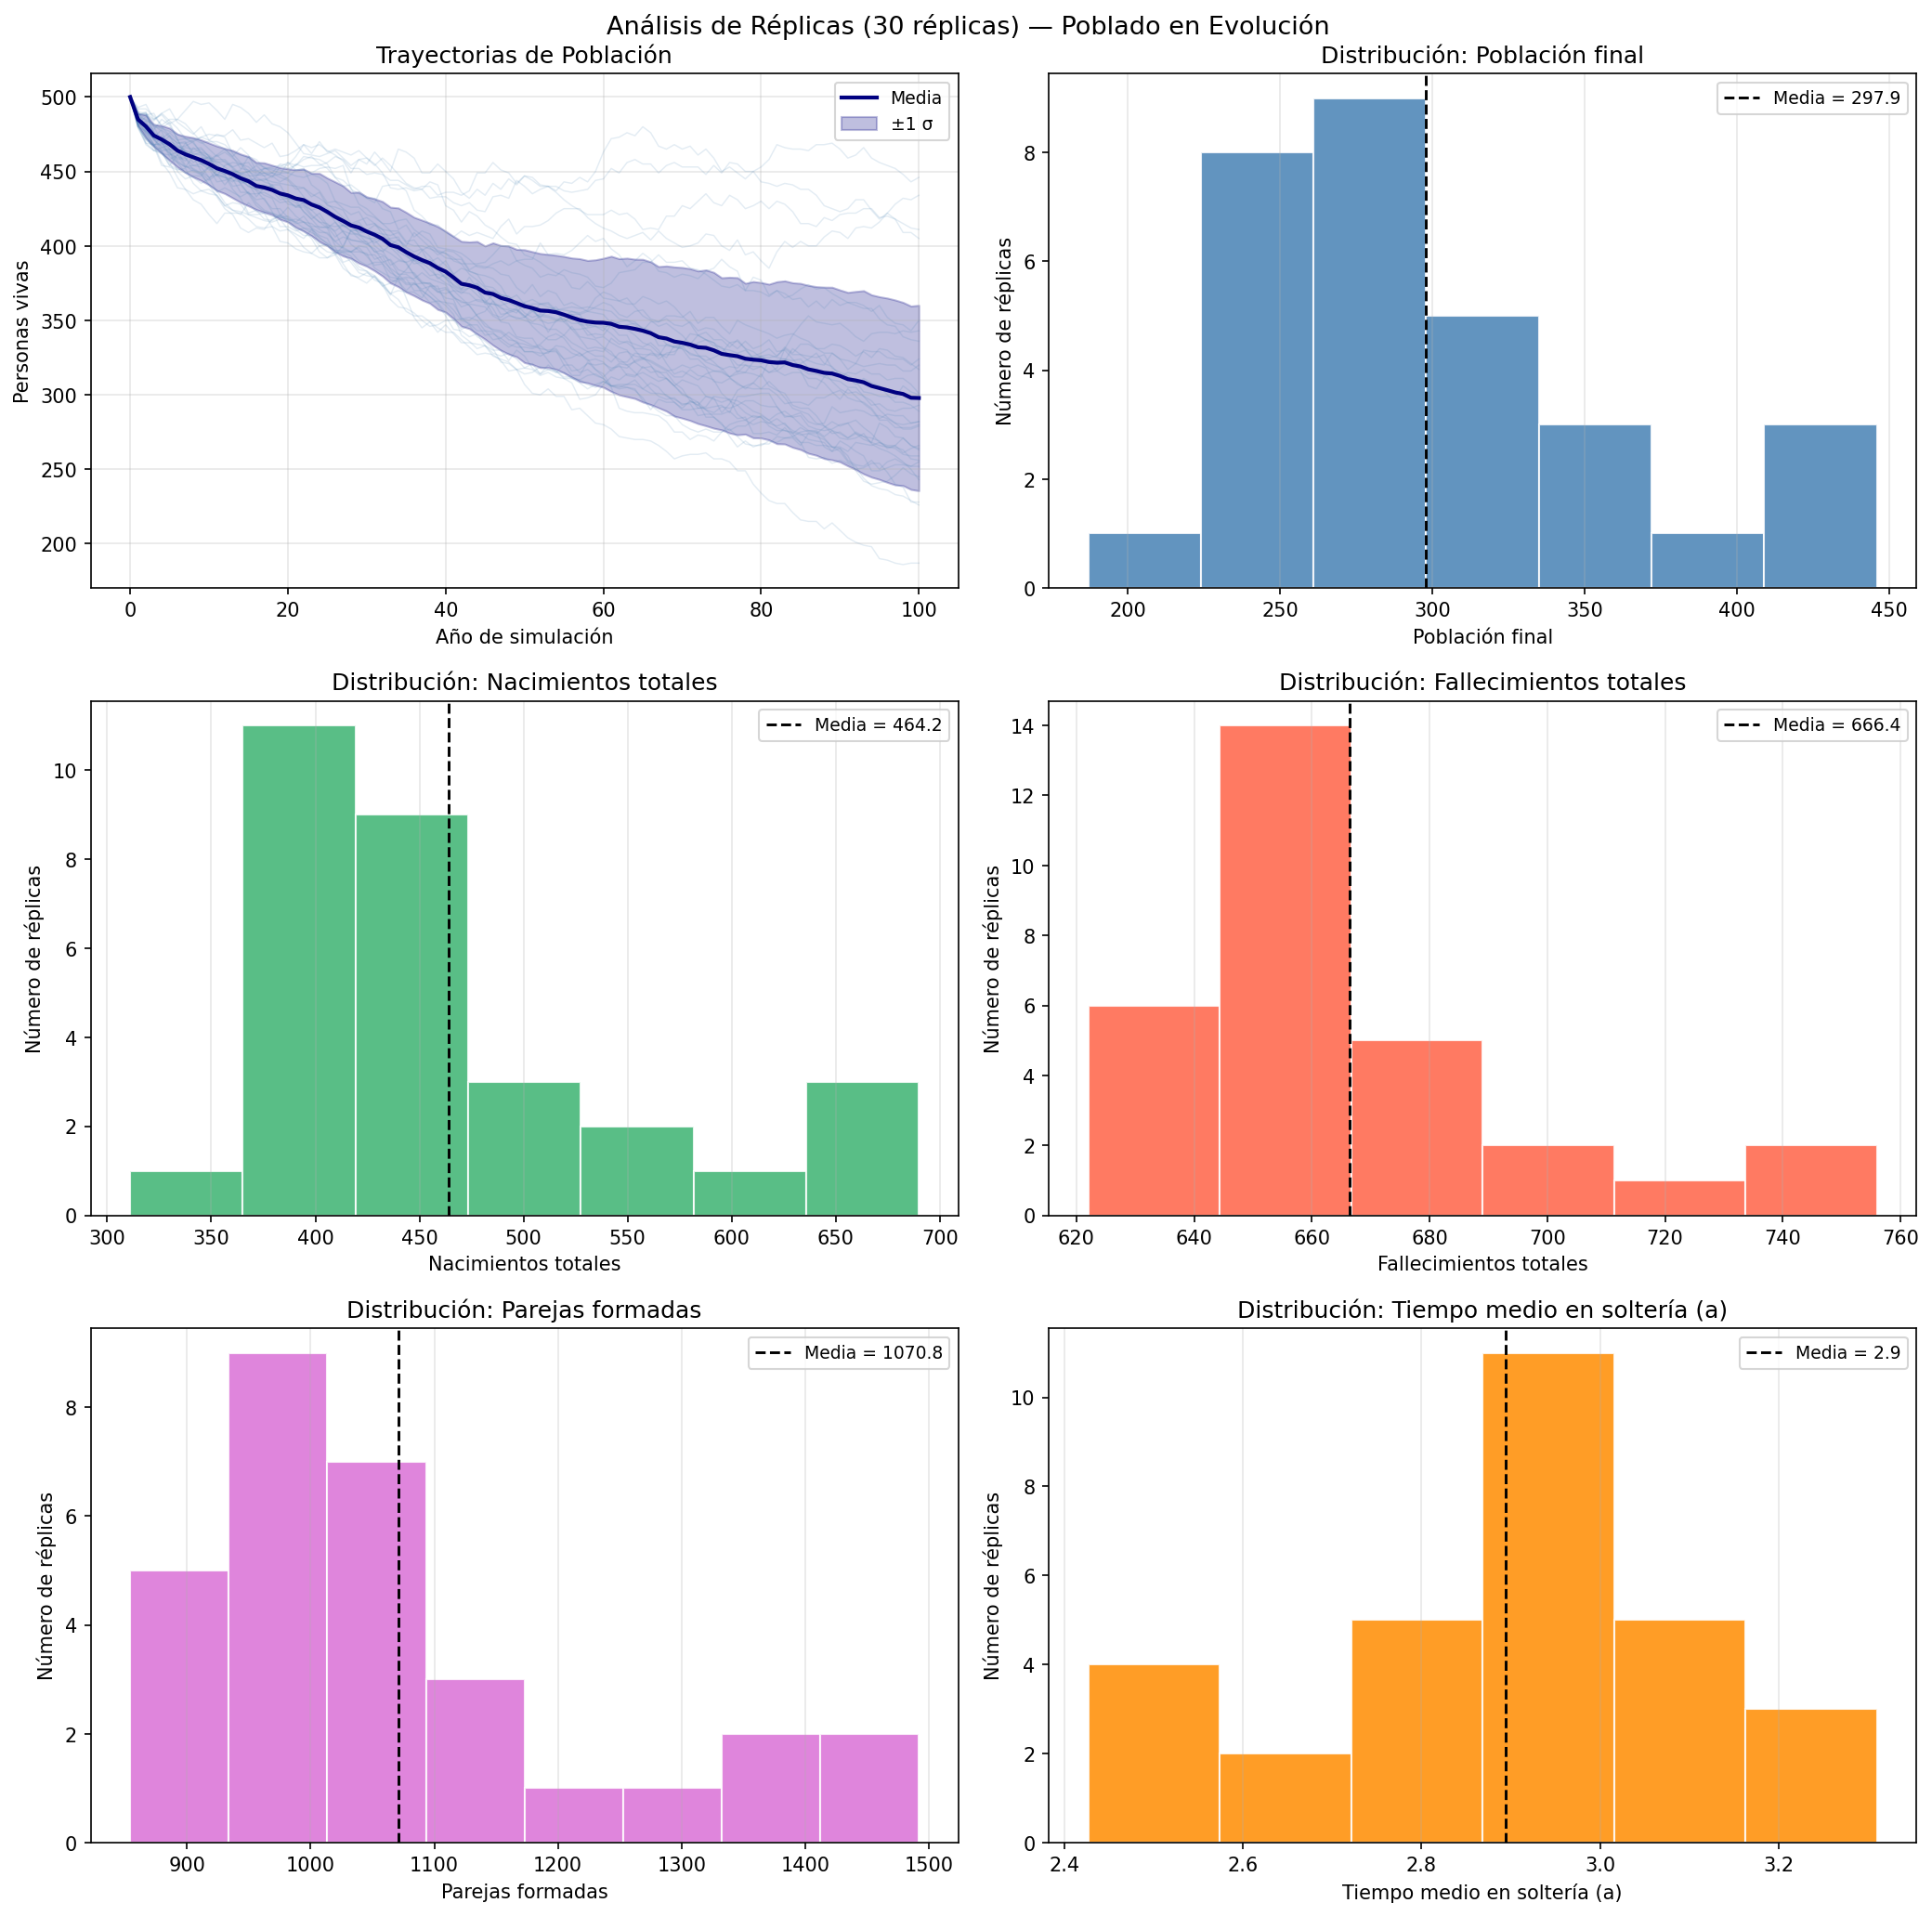
\includegraphics[width=\linewidth]{figures/batch_h100_m400.png}
  \caption{Análisis de 30 réplicas: $H=100$, $M=400$.}
  \label{fig:batch_h100_m400}
\end{figure}

% =============================================================================
\end{document}
